% MO433 report. Numbers come from generated/macros.tex and generated/*.tex (written by
% `mo433 report` from results.csv and report/data/; never edit them) or are traceable to a
% committed file named in a comment next to them. Layout follows the course format
% (https://www.ic.unicamp.br/~afalcao/mo433/node5.html): Letter, 11pt; cover page with course,
% name, RA, delivery date and a summary of techniques and results; conclusion and suggestions
% for improvement on the final page. Build: latexmk -pdf main.tex
\documentclass[letterpaper,11pt]{article}
\usepackage[letterpaper,margin=2cm]{geometry}
\usepackage[T1]{fontenc}
\usepackage[utf8]{inputenc}
\usepackage{booktabs}
\usepackage{graphicx}
\usepackage{amsmath}
\usepackage{xcolor}
\usepackage[numbers,sort&compress]{natbib}
\usepackage[hidelinks]{hyperref}

% Generated by `mo433 report` from results.csv and report/data/. Do not edit.
\newcommand{\AccASKnnOne}{19.2}
\newcommand{\AccSdASKnnOne}{0.5}
\newcommand{\AccASKnnOneSeedZero}{18.8}
\newcommand{\AccASKnnOneSeedOne}{19.2}
\newcommand{\AccASKnnOneSeedTwo}{19.7}
\newcommand{\AccASKnnTen}{25.1}
\newcommand{\AccSdASKnnTen}{1.8}
\newcommand{\AccASKnnTenSeedZero}{23.9}
\newcommand{\AccASKnnTenSeedOne}{24.2}
\newcommand{\AccASKnnTenSeedTwo}{27.1}
\newcommand{\AccASKnnFifty}{29.8}
\newcommand{\AccSdASKnnFifty}{1.5}
\newcommand{\AccASKnnFiftySeedZero}{28.5}
\newcommand{\AccASKnnFiftySeedOne}{29.5}
\newcommand{\AccASKnnFiftySeedTwo}{31.5}
\newcommand{\AccASKnnHundred}{31.1}
\newcommand{\AccSdASKnnHundred}{1.3}
\newcommand{\AccASKnnHundredSeedZero}{29.8}
\newcommand{\AccASKnnHundredSeedOne}{31.0}
\newcommand{\AccASKnnHundredSeedTwo}{32.4}
\newcommand{\AccASLinOne}{19.8}
\newcommand{\AccSdASLinOne}{1.3}
\newcommand{\AccASLinOneSeedZero}{18.3}
\newcommand{\AccASLinOneSeedOne}{20.4}
\newcommand{\AccASLinOneSeedTwo}{20.7}
\newcommand{\AccASLinTen}{26.8}
\newcommand{\AccSdASLinTen}{1.0}
\newcommand{\AccASLinTenSeedZero}{25.8}
\newcommand{\AccASLinTenSeedOne}{26.8}
\newcommand{\AccASLinTenSeedTwo}{27.8}
\newcommand{\AccASLinFifty}{33.0}
\newcommand{\AccSdASLinFifty}{0.9}
\newcommand{\AccASLinFiftySeedZero}{32.1}
\newcommand{\AccASLinFiftySeedOne}{32.9}
\newcommand{\AccASLinFiftySeedTwo}{33.9}
\newcommand{\AccASLinHundred}{35.0}
\newcommand{\AccSdASLinHundred}{1.1}
\newcommand{\AccASLinHundredSeedZero}{33.8}
\newcommand{\AccASLinHundredSeedOne}{35.0}
\newcommand{\AccASLinHundredSeedTwo}{36.1}
\newcommand{\AccASRbfOne}{21.0}
\newcommand{\AccSdASRbfOne}{1.4}
\newcommand{\AccASRbfOneSeedZero}{19.8}
\newcommand{\AccASRbfOneSeedOne}{20.8}
\newcommand{\AccASRbfOneSeedTwo}{22.4}
\newcommand{\AccASRbfTen}{30.2}
\newcommand{\AccSdASRbfTen}{1.7}
\newcommand{\AccASRbfTenSeedZero}{28.4}
\newcommand{\AccASRbfTenSeedOne}{30.6}
\newcommand{\AccASRbfTenSeedTwo}{31.7}
\newcommand{\AccASRbfFifty}{35.9}
\newcommand{\AccSdASRbfFifty}{1.2}
\newcommand{\AccASRbfFiftySeedZero}{34.6}
\newcommand{\AccASRbfFiftySeedOne}{36.0}
\newcommand{\AccASRbfFiftySeedTwo}{37.0}
\newcommand{\AccASRbfHundred}{37.7}
\newcommand{\AccSdASRbfHundred}{1.3}
\newcommand{\AccASRbfHundredSeedZero}{36.2}
\newcommand{\AccASRbfHundredSeedOne}{38.2}
\newcommand{\AccASRbfHundredSeedTwo}{38.8}
\newcommand{\AccBSFullKnnOne}{59.5}
\newcommand{\AccSdBSFullKnnOne}{0.8}
\newcommand{\AccBSFullKnnOneSeedZero}{60.4}
\newcommand{\AccBSFullKnnOneSeedOne}{59.1}
\newcommand{\AccBSFullKnnOneSeedTwo}{59.1}
\newcommand{\AccBSFullKnnTen}{73.7}
\newcommand{\AccSdBSFullKnnTen}{0.1}
\newcommand{\AccBSFullKnnTenSeedZero}{73.8}
\newcommand{\AccBSFullKnnTenSeedOne}{73.7}
\newcommand{\AccBSFullKnnTenSeedTwo}{73.5}
\newcommand{\AccBSFullKnnFifty}{77.1}
\newcommand{\AccSdBSFullKnnFifty}{0.1}
\newcommand{\AccBSFullKnnFiftySeedZero}{77.1}
\newcommand{\AccBSFullKnnFiftySeedOne}{77.2}
\newcommand{\AccBSFullKnnFiftySeedTwo}{77.0}
\newcommand{\AccBSFullKnnHundred}{78.4}
\newcommand{\AccSdBSFullKnnHundred}{0.3}
\newcommand{\AccBSFullKnnHundredSeedZero}{78.7}
\newcommand{\AccBSFullKnnHundredSeedOne}{78.2}
\newcommand{\AccBSFullKnnHundredSeedTwo}{78.3}
\newcommand{\AccBSFullLinOne}{64.9}
\newcommand{\AccSdBSFullLinOne}{0.7}
\newcommand{\AccBSFullLinOneSeedZero}{65.5}
\newcommand{\AccBSFullLinOneSeedOne}{64.1}
\newcommand{\AccBSFullLinOneSeedTwo}{64.9}
\newcommand{\AccBSFullLinTen}{76.2}
\newcommand{\AccSdBSFullLinTen}{0.2}
\newcommand{\AccBSFullLinTenSeedZero}{76.4}
\newcommand{\AccBSFullLinTenSeedOne}{76.0}
\newcommand{\AccBSFullLinTenSeedTwo}{76.1}
\newcommand{\AccBSFullLinFifty}{80.5}
\newcommand{\AccSdBSFullLinFifty}{0.4}
\newcommand{\AccBSFullLinFiftySeedZero}{81.0}
\newcommand{\AccBSFullLinFiftySeedOne}{80.2}
\newcommand{\AccBSFullLinFiftySeedTwo}{80.4}
\newcommand{\AccBSFullLinHundred}{81.7}
\newcommand{\AccSdBSFullLinHundred}{0.4}
\newcommand{\AccBSFullLinHundredSeedZero}{82.2}
\newcommand{\AccBSFullLinHundredSeedOne}{81.5}
\newcommand{\AccBSFullLinHundredSeedTwo}{81.6}
\newcommand{\AccBSFullRbfOne}{64.0}
\newcommand{\AccSdBSFullRbfOne}{0.5}
\newcommand{\AccBSFullRbfOneSeedZero}{64.2}
\newcommand{\AccBSFullRbfOneSeedOne}{63.5}
\newcommand{\AccBSFullRbfOneSeedTwo}{64.3}
\newcommand{\AccBSFullRbfTen}{76.0}
\newcommand{\AccSdBSFullRbfTen}{0.1}
\newcommand{\AccBSFullRbfTenSeedZero}{76.0}
\newcommand{\AccBSFullRbfTenSeedOne}{76.1}
\newcommand{\AccBSFullRbfTenSeedTwo}{75.9}
\newcommand{\AccBSFullRbfFifty}{81.0}
\newcommand{\AccSdBSFullRbfFifty}{0.4}
\newcommand{\AccBSFullRbfFiftySeedZero}{81.4}
\newcommand{\AccBSFullRbfFiftySeedOne}{80.7}
\newcommand{\AccBSFullRbfFiftySeedTwo}{80.9}
\newcommand{\AccBSFullRbfHundred}{82.7}
\newcommand{\AccSdBSFullRbfHundred}{0.4}
\newcommand{\AccBSFullRbfHundredSeedZero}{83.1}
\newcommand{\AccBSFullRbfHundredSeedOne}{82.4}
\newcommand{\AccBSFullRbfHundredSeedTwo}{82.5}
\newcommand{\AccCSFullKnnOne}{73.8}
\newcommand{\AccSdCSFullKnnOne}{0.9}
\newcommand{\AccCSFullKnnOneSeedZero}{73.1}
\newcommand{\AccCSFullKnnOneSeedOne}{74.8}
\newcommand{\AccCSFullKnnOneSeedTwo}{73.5}
\newcommand{\AccCSFullKnnTen}{86.8}
\newcommand{\AccSdCSFullKnnTen}{0.2}
\newcommand{\AccCSFullKnnTenSeedZero}{86.7}
\newcommand{\AccCSFullKnnTenSeedOne}{87.0}
\newcommand{\AccCSFullKnnTenSeedTwo}{86.7}
\newcommand{\AccCSFullKnnFifty}{90.9}
\newcommand{\AccSdCSFullKnnFifty}{0.2}
\newcommand{\AccCSFullKnnFiftySeedZero}{90.9}
\newcommand{\AccCSFullKnnFiftySeedOne}{91.0}
\newcommand{\AccCSFullKnnFiftySeedTwo}{90.7}
\newcommand{\AccCSFullKnnHundred}{92.1}
\newcommand{\AccSdCSFullKnnHundred}{0.1}
\newcommand{\AccCSFullKnnHundredSeedZero}{92.0}
\newcommand{\AccCSFullKnnHundredSeedOne}{92.2}
\newcommand{\AccCSFullKnnHundredSeedTwo}{92.0}
\newcommand{\AccCSFullLinOne}{81.9}
\newcommand{\AccSdCSFullLinOne}{0.1}
\newcommand{\AccCSFullLinOneSeedZero}{82.1}
\newcommand{\AccCSFullLinOneSeedOne}{81.8}
\newcommand{\AccCSFullLinOneSeedTwo}{81.9}
\newcommand{\AccCSFullLinTen}{91.1}
\newcommand{\AccSdCSFullLinTen}{0.2}
\newcommand{\AccCSFullLinTenSeedZero}{91.3}
\newcommand{\AccCSFullLinTenSeedOne}{90.9}
\newcommand{\AccCSFullLinTenSeedTwo}{91.1}
\newcommand{\AccCSFullLinFifty}{93.4}
\newcommand{\AccSdCSFullLinFifty}{0.1}
\newcommand{\AccCSFullLinFiftySeedZero}{93.4}
\newcommand{\AccCSFullLinFiftySeedOne}{93.3}
\newcommand{\AccCSFullLinFiftySeedTwo}{93.5}
\newcommand{\AccCSFullLinHundred}{93.9}
\newcommand{\AccSdCSFullLinHundred}{0.2}
\newcommand{\AccCSFullLinHundredSeedZero}{94.0}
\newcommand{\AccCSFullLinHundredSeedOne}{93.7}
\newcommand{\AccCSFullLinHundredSeedTwo}{94.0}
\newcommand{\AccCSFullRbfOne}{78.1}
\newcommand{\AccSdCSFullRbfOne}{0.6}
\newcommand{\AccCSFullRbfOneSeedZero}{77.4}
\newcommand{\AccCSFullRbfOneSeedOne}{78.7}
\newcommand{\AccCSFullRbfOneSeedTwo}{78.2}
\newcommand{\AccCSFullRbfTen}{90.2}
\newcommand{\AccSdCSFullRbfTen}{0.1}
\newcommand{\AccCSFullRbfTenSeedZero}{90.3}
\newcommand{\AccCSFullRbfTenSeedOne}{90.1}
\newcommand{\AccCSFullRbfTenSeedTwo}{90.3}
\newcommand{\AccCSFullRbfFifty}{93.3}
\newcommand{\AccSdCSFullRbfFifty}{0.1}
\newcommand{\AccCSFullRbfFiftySeedZero}{93.2}
\newcommand{\AccCSFullRbfFiftySeedOne}{93.3}
\newcommand{\AccCSFullRbfFiftySeedTwo}{93.3}
\newcommand{\AccCSFullRbfHundred}{94.0}
\newcommand{\AccSdCSFullRbfHundred}{0.1}
\newcommand{\AccCSFullRbfHundredSeedZero}{94.0}
\newcommand{\AccCSFullRbfHundredSeedOne}{94.0}
\newcommand{\AccCSFullRbfHundredSeedTwo}{94.1}
\newcommand{\AccBSHalfKnnOne}{56.9}
\newcommand{\AccSdBSHalfKnnOne}{0.3}
\newcommand{\AccBSHalfKnnOneSeedZero}{56.7}
\newcommand{\AccBSHalfKnnOneSeedOne}{57.3}
\newcommand{\AccBSHalfKnnOneSeedTwo}{56.9}
\newcommand{\AccBSHalfKnnTen}{70.1}
\newcommand{\AccSdBSHalfKnnTen}{0.5}
\newcommand{\AccBSHalfKnnTenSeedZero}{70.1}
\newcommand{\AccBSHalfKnnTenSeedOne}{69.7}
\newcommand{\AccBSHalfKnnTenSeedTwo}{70.6}
\newcommand{\AccBSHalfKnnFifty}{73.9}
\newcommand{\AccSdBSHalfKnnFifty}{0.4}
\newcommand{\AccBSHalfKnnFiftySeedZero}{73.8}
\newcommand{\AccBSHalfKnnFiftySeedOne}{73.5}
\newcommand{\AccBSHalfKnnFiftySeedTwo}{74.3}
\newcommand{\AccBSHalfKnnHundred}{75.2}
\newcommand{\AccSdBSHalfKnnHundred}{0.1}
\newcommand{\AccBSHalfKnnHundredSeedZero}{75.1}
\newcommand{\AccBSHalfKnnHundredSeedOne}{75.1}
\newcommand{\AccBSHalfKnnHundredSeedTwo}{75.3}
\newcommand{\AccBSHalfLinOne}{62.7}
\newcommand{\AccSdBSHalfLinOne}{0.2}
\newcommand{\AccBSHalfLinOneSeedZero}{62.5}
\newcommand{\AccBSHalfLinOneSeedOne}{62.7}
\newcommand{\AccBSHalfLinOneSeedTwo}{62.9}
\newcommand{\AccBSHalfLinTen}{72.6}
\newcommand{\AccSdBSHalfLinTen}{0.3}
\newcommand{\AccBSHalfLinTenSeedZero}{72.4}
\newcommand{\AccBSHalfLinTenSeedOne}{72.5}
\newcommand{\AccBSHalfLinTenSeedTwo}{72.9}
\newcommand{\AccBSHalfLinFifty}{77.5}
\newcommand{\AccSdBSHalfLinFifty}{0.3}
\newcommand{\AccBSHalfLinFiftySeedZero}{77.2}
\newcommand{\AccBSHalfLinFiftySeedOne}{77.5}
\newcommand{\AccBSHalfLinFiftySeedTwo}{77.7}
\newcommand{\AccBSHalfLinHundred}{78.7}
\newcommand{\AccSdBSHalfLinHundred}{0.2}
\newcommand{\AccBSHalfLinHundredSeedZero}{78.4}
\newcommand{\AccBSHalfLinHundredSeedOne}{78.8}
\newcommand{\AccBSHalfLinHundredSeedTwo}{78.9}
\newcommand{\AccBSHalfRbfOne}{62.0}
\newcommand{\AccSdBSHalfRbfOne}{0.2}
\newcommand{\AccBSHalfRbfOneSeedZero}{62.2}
\newcommand{\AccBSHalfRbfOneSeedOne}{61.7}
\newcommand{\AccBSHalfRbfOneSeedTwo}{62.2}
\newcommand{\AccBSHalfRbfTen}{72.7}
\newcommand{\AccSdBSHalfRbfTen}{0.5}
\newcommand{\AccBSHalfRbfTenSeedZero}{72.6}
\newcommand{\AccBSHalfRbfTenSeedOne}{72.3}
\newcommand{\AccBSHalfRbfTenSeedTwo}{73.3}
\newcommand{\AccBSHalfRbfFifty}{78.0}
\newcommand{\AccSdBSHalfRbfFifty}{0.1}
\newcommand{\AccBSHalfRbfFiftySeedZero}{77.9}
\newcommand{\AccBSHalfRbfFiftySeedOne}{78.0}
\newcommand{\AccBSHalfRbfFiftySeedTwo}{78.2}
\newcommand{\AccBSHalfRbfHundred}{79.7}
\newcommand{\AccSdBSHalfRbfHundred}{0.2}
\newcommand{\AccBSHalfRbfHundredSeedZero}{79.7}
\newcommand{\AccBSHalfRbfHundredSeedOne}{79.5}
\newcommand{\AccBSHalfRbfHundredSeedTwo}{79.9}
\newcommand{\AccCSHalfKnnOne}{71.7}
\newcommand{\AccSdCSHalfKnnOne}{0.8}
\newcommand{\AccCSHalfKnnOneSeedZero}{71.7}
\newcommand{\AccCSHalfKnnOneSeedOne}{72.5}
\newcommand{\AccCSHalfKnnOneSeedTwo}{70.8}
\newcommand{\AccCSHalfKnnTen}{85.4}
\newcommand{\AccSdCSHalfKnnTen}{0.3}
\newcommand{\AccCSHalfKnnTenSeedZero}{85.4}
\newcommand{\AccCSHalfKnnTenSeedOne}{85.6}
\newcommand{\AccCSHalfKnnTenSeedTwo}{85.1}
\newcommand{\AccCSHalfKnnFifty}{89.5}
\newcommand{\AccSdCSHalfKnnFifty}{0.1}
\newcommand{\AccCSHalfKnnFiftySeedZero}{89.4}
\newcommand{\AccCSHalfKnnFiftySeedOne}{89.4}
\newcommand{\AccCSHalfKnnFiftySeedTwo}{89.6}
\newcommand{\AccCSHalfKnnHundred}{91.0}
\newcommand{\AccSdCSHalfKnnHundred}{0.2}
\newcommand{\AccCSHalfKnnHundredSeedZero}{90.8}
\newcommand{\AccCSHalfKnnHundredSeedOne}{90.9}
\newcommand{\AccCSHalfKnnHundredSeedTwo}{91.2}
\newcommand{\AccCSHalfLinOne}{79.8}
\newcommand{\AccSdCSHalfLinOne}{0.9}
\newcommand{\AccCSHalfLinOneSeedZero}{80.5}
\newcommand{\AccCSHalfLinOneSeedOne}{80.1}
\newcommand{\AccCSHalfLinOneSeedTwo}{78.9}
\newcommand{\AccCSHalfLinTen}{89.7}
\newcommand{\AccSdCSHalfLinTen}{0.2}
\newcommand{\AccCSHalfLinTenSeedZero}{89.5}
\newcommand{\AccCSHalfLinTenSeedOne}{89.8}
\newcommand{\AccCSHalfLinTenSeedTwo}{89.8}
\newcommand{\AccCSHalfLinFifty}{92.1}
\newcommand{\AccSdCSHalfLinFifty}{0.1}
\newcommand{\AccCSHalfLinFiftySeedZero}{92.0}
\newcommand{\AccCSHalfLinFiftySeedOne}{92.2}
\newcommand{\AccCSHalfLinFiftySeedTwo}{92.1}
\newcommand{\AccCSHalfLinHundred}{92.8}
\newcommand{\AccSdCSHalfLinHundred}{0.1}
\newcommand{\AccCSHalfLinHundredSeedZero}{92.8}
\newcommand{\AccCSHalfLinHundredSeedOne}{92.8}
\newcommand{\AccCSHalfLinHundredSeedTwo}{92.7}
\newcommand{\AccCSHalfRbfOne}{76.8}
\newcommand{\AccSdCSHalfRbfOne}{0.3}
\newcommand{\AccCSHalfRbfOneSeedZero}{76.8}
\newcommand{\AccCSHalfRbfOneSeedOne}{77.1}
\newcommand{\AccCSHalfRbfOneSeedTwo}{76.5}
\newcommand{\AccCSHalfRbfTen}{88.9}
\newcommand{\AccSdCSHalfRbfTen}{0.1}
\newcommand{\AccCSHalfRbfTenSeedZero}{88.8}
\newcommand{\AccCSHalfRbfTenSeedOne}{89.0}
\newcommand{\AccCSHalfRbfTenSeedTwo}{88.9}
\newcommand{\AccCSHalfRbfFifty}{92.3}
\newcommand{\AccSdCSHalfRbfFifty}{0.1}
\newcommand{\AccCSHalfRbfFiftySeedZero}{92.4}
\newcommand{\AccCSHalfRbfFiftySeedOne}{92.2}
\newcommand{\AccCSHalfRbfFiftySeedTwo}{92.3}
\newcommand{\AccCSHalfRbfHundred}{93.4}
\newcommand{\AccSdCSHalfRbfHundred}{0.1}
\newcommand{\AccCSHalfRbfHundredSeedZero}{93.3}
\newcommand{\AccCSHalfRbfHundredSeedOne}{93.4}
\newcommand{\AccCSHalfRbfHundredSeedTwo}{93.3}
\newcommand{\AccALKnnOne}{20.5}
\newcommand{\AccSdALKnnOne}{0.3}
\newcommand{\AccALKnnOneSeedZero}{20.4}
\newcommand{\AccALKnnOneSeedOne}{20.7}
\newcommand{\AccALKnnTen}{26.5}
\newcommand{\AccSdALKnnTen}{1.2}
\newcommand{\AccALKnnTenSeedZero}{25.7}
\newcommand{\AccALKnnTenSeedOne}{27.4}
\newcommand{\AccALKnnFifty}{31.6}
\newcommand{\AccSdALKnnFifty}{0.4}
\newcommand{\AccALKnnFiftySeedZero}{31.3}
\newcommand{\AccALKnnFiftySeedOne}{31.9}
\newcommand{\AccALKnnHundred}{33.3}
\newcommand{\AccSdALKnnHundred}{0.2}
\newcommand{\AccALKnnHundredSeedZero}{33.5}
\newcommand{\AccALKnnHundredSeedOne}{33.2}
\newcommand{\AccALLinOne}{21.7}
\newcommand{\AccSdALLinOne}{0.1}
\newcommand{\AccALLinOneSeedZero}{21.7}
\newcommand{\AccALLinOneSeedOne}{21.8}
\newcommand{\AccALLinTen}{27.7}
\newcommand{\AccSdALLinTen}{1.1}
\newcommand{\AccALLinTenSeedZero}{28.5}
\newcommand{\AccALLinTenSeedOne}{26.9}
\newcommand{\AccALLinFifty}{34.7}
\newcommand{\AccSdALLinFifty}{1.4}
\newcommand{\AccALLinFiftySeedZero}{35.6}
\newcommand{\AccALLinFiftySeedOne}{33.7}
\newcommand{\AccALLinHundred}{37.6}
\newcommand{\AccSdALLinHundred}{0.5}
\newcommand{\AccALLinHundredSeedZero}{38.0}
\newcommand{\AccALLinHundredSeedOne}{37.3}
\newcommand{\AccALRbfOne}{23.3}
\newcommand{\AccSdALRbfOne}{0.2}
\newcommand{\AccALRbfOneSeedZero}{23.2}
\newcommand{\AccALRbfOneSeedOne}{23.5}
\newcommand{\AccALRbfTen}{33.3}
\newcommand{\AccSdALRbfTen}{0.2}
\newcommand{\AccALRbfTenSeedZero}{33.2}
\newcommand{\AccALRbfTenSeedOne}{33.5}
\newcommand{\AccALRbfFifty}{39.9}
\newcommand{\AccSdALRbfFifty}{0.0}
\newcommand{\AccALRbfFiftySeedZero}{39.9}
\newcommand{\AccALRbfFiftySeedOne}{39.9}
\newcommand{\AccALRbfHundred}{42.1}
\newcommand{\AccSdALRbfHundred}{0.1}
\newcommand{\AccALRbfHundredSeedZero}{42.2}
\newcommand{\AccALRbfHundredSeedOne}{42.0}
\newcommand{\AccBLFullKnnOne}{64.0}
\newcommand{\AccSdBLFullKnnOne}{0.1}
\newcommand{\AccBLFullKnnOneSeedZero}{63.9}
\newcommand{\AccBLFullKnnOneSeedOne}{64.1}
\newcommand{\AccBLFullKnnTen}{78.1}
\newcommand{\AccSdBLFullKnnTen}{0.0}
\newcommand{\AccBLFullKnnTenSeedZero}{78.1}
\newcommand{\AccBLFullKnnTenSeedOne}{78.1}
\newcommand{\AccBLFullKnnFifty}{81.3}
\newcommand{\AccSdBLFullKnnFifty}{0.0}
\newcommand{\AccBLFullKnnFiftySeedZero}{81.3}
\newcommand{\AccBLFullKnnFiftySeedOne}{81.3}
\newcommand{\AccBLFullKnnHundred}{82.1}
\newcommand{\AccSdBLFullKnnHundred}{0.0}
\newcommand{\AccBLFullKnnHundredSeedZero}{82.2}
\newcommand{\AccBLFullKnnHundredSeedOne}{82.1}
\newcommand{\AccBLFullLinOne}{70.4}
\newcommand{\AccSdBLFullLinOne}{0.0}
\newcommand{\AccBLFullLinOneSeedZero}{70.4}
\newcommand{\AccBLFullLinOneSeedOne}{70.4}
\newcommand{\AccBLFullLinTen}{80.2}
\newcommand{\AccSdBLFullLinTen}{0.0}
\newcommand{\AccBLFullLinTenSeedZero}{80.2}
\newcommand{\AccBLFullLinTenSeedOne}{80.2}
\newcommand{\AccBLFullLinFifty}{83.7}
\newcommand{\AccSdBLFullLinFifty}{0.1}
\newcommand{\AccBLFullLinFiftySeedZero}{83.8}
\newcommand{\AccBLFullLinFiftySeedOne}{83.7}
\newcommand{\AccBLFullLinHundred}{84.9}
\newcommand{\AccSdBLFullLinHundred}{0.2}
\newcommand{\AccBLFullLinHundredSeedZero}{85.0}
\newcommand{\AccBLFullLinHundredSeedOne}{84.8}
\newcommand{\AccBLFullRbfOne}{67.1}
\newcommand{\AccSdBLFullRbfOne}{0.8}
\newcommand{\AccBLFullRbfOneSeedZero}{67.7}
\newcommand{\AccBLFullRbfOneSeedOne}{66.5}
\newcommand{\AccBLFullRbfTen}{80.0}
\newcommand{\AccSdBLFullRbfTen}{0.2}
\newcommand{\AccBLFullRbfTenSeedZero}{80.2}
\newcommand{\AccBLFullRbfTenSeedOne}{79.9}
\newcommand{\AccBLFullRbfFifty}{84.6}
\newcommand{\AccSdBLFullRbfFifty}{0.1}
\newcommand{\AccBLFullRbfFiftySeedZero}{84.7}
\newcommand{\AccBLFullRbfFiftySeedOne}{84.5}
\newcommand{\AccBLFullRbfHundred}{86.4}
\newcommand{\AccSdBLFullRbfHundred}{0.4}
\newcommand{\AccBLFullRbfHundredSeedZero}{86.7}
\newcommand{\AccBLFullRbfHundredSeedOne}{86.1}
\newcommand{\AccCLFullKnnOne}{77.4}
\newcommand{\AccSdCLFullKnnOne}{0.4}
\newcommand{\AccCLFullKnnOneSeedZero}{77.7}
\newcommand{\AccCLFullKnnOneSeedOne}{77.1}
\newcommand{\AccCLFullKnnTen}{90.1}
\newcommand{\AccSdCLFullKnnTen}{0.1}
\newcommand{\AccCLFullKnnTenSeedZero}{90.0}
\newcommand{\AccCLFullKnnTenSeedOne}{90.2}
\newcommand{\AccCLFullKnnFifty}{93.9}
\newcommand{\AccSdCLFullKnnFifty}{0.3}
\newcommand{\AccCLFullKnnFiftySeedZero}{93.7}
\newcommand{\AccCLFullKnnFiftySeedOne}{94.1}
\newcommand{\AccCLFullKnnHundred}{94.7}
\newcommand{\AccSdCLFullKnnHundred}{0.1}
\newcommand{\AccCLFullKnnHundredSeedZero}{94.6}
\newcommand{\AccCLFullKnnHundredSeedOne}{94.7}
\newcommand{\AccCLFullLinOne}{85.9}
\newcommand{\AccSdCLFullLinOne}{0.7}
\newcommand{\AccCLFullLinOneSeedZero}{85.5}
\newcommand{\AccCLFullLinOneSeedOne}{86.4}
\newcommand{\AccCLFullLinTen}{94.7}
\newcommand{\AccSdCLFullLinTen}{0.2}
\newcommand{\AccCLFullLinTenSeedZero}{94.5}
\newcommand{\AccCLFullLinTenSeedOne}{94.8}
\newcommand{\AccCLFullLinFifty}{96.2}
\newcommand{\AccSdCLFullLinFifty}{0.2}
\newcommand{\AccCLFullLinFiftySeedZero}{96.1}
\newcommand{\AccCLFullLinFiftySeedOne}{96.3}
\newcommand{\AccCLFullLinHundred}{96.6}
\newcommand{\AccSdCLFullLinHundred}{0.1}
\newcommand{\AccCLFullLinHundredSeedZero}{96.5}
\newcommand{\AccCLFullLinHundredSeedOne}{96.6}
\newcommand{\AccCLFullRbfOne}{80.7}
\newcommand{\AccSdCLFullRbfOne}{0.3}
\newcommand{\AccCLFullRbfOneSeedZero}{80.5}
\newcommand{\AccCLFullRbfOneSeedOne}{81.0}
\newcommand{\AccCLFullRbfTen}{93.5}
\newcommand{\AccSdCLFullRbfTen}{0.2}
\newcommand{\AccCLFullRbfTenSeedZero}{93.3}
\newcommand{\AccCLFullRbfTenSeedOne}{93.6}
\newcommand{\AccCLFullRbfFifty}{96.0}
\newcommand{\AccSdCLFullRbfFifty}{0.2}
\newcommand{\AccCLFullRbfFiftySeedZero}{95.9}
\newcommand{\AccCLFullRbfFiftySeedOne}{96.1}
\newcommand{\AccCLFullRbfHundred}{96.5}
\newcommand{\AccSdCLFullRbfHundred}{0.0}
\newcommand{\AccCLFullRbfHundredSeedZero}{96.5}
\newcommand{\AccCLFullRbfHundredSeedOne}{96.5}
\newcommand{\AccBLHalfKnnOne}{60.5}
\newcommand{\AccSdBLHalfKnnOne}{0.9}
\newcommand{\AccBLHalfKnnOneSeedZero}{61.1}
\newcommand{\AccBLHalfKnnOneSeedOne}{59.9}
\newcommand{\AccBLHalfKnnTen}{74.1}
\newcommand{\AccSdBLHalfKnnTen}{0.2}
\newcommand{\AccBLHalfKnnTenSeedZero}{74.3}
\newcommand{\AccBLHalfKnnTenSeedOne}{73.9}
\newcommand{\AccBLHalfKnnFifty}{77.5}
\newcommand{\AccSdBLHalfKnnFifty}{0.2}
\newcommand{\AccBLHalfKnnFiftySeedZero}{77.7}
\newcommand{\AccBLHalfKnnFiftySeedOne}{77.4}
\newcommand{\AccBLHalfKnnHundred}{78.6}
\newcommand{\AccSdBLHalfKnnHundred}{0.4}
\newcommand{\AccBLHalfKnnHundredSeedZero}{78.9}
\newcommand{\AccBLHalfKnnHundredSeedOne}{78.3}
\newcommand{\AccBLHalfLinOne}{65.4}
\newcommand{\AccSdBLHalfLinOne}{0.6}
\newcommand{\AccBLHalfLinOneSeedZero}{65.8}
\newcommand{\AccBLHalfLinOneSeedOne}{65.0}
\newcommand{\AccBLHalfLinTen}{75.3}
\newcommand{\AccSdBLHalfLinTen}{0.1}
\newcommand{\AccBLHalfLinTenSeedZero}{75.4}
\newcommand{\AccBLHalfLinTenSeedOne}{75.3}
\newcommand{\AccBLHalfLinFifty}{80.0}
\newcommand{\AccSdBLHalfLinFifty}{0.4}
\newcommand{\AccBLHalfLinFiftySeedZero}{80.3}
\newcommand{\AccBLHalfLinFiftySeedOne}{79.7}
\newcommand{\AccBLHalfLinHundred}{81.6}
\newcommand{\AccSdBLHalfLinHundred}{0.1}
\newcommand{\AccBLHalfLinHundredSeedZero}{81.7}
\newcommand{\AccBLHalfLinHundredSeedOne}{81.5}
\newcommand{\AccBLHalfRbfOne}{64.3}
\newcommand{\AccSdBLHalfRbfOne}{0.7}
\newcommand{\AccBLHalfRbfOneSeedZero}{64.8}
\newcommand{\AccBLHalfRbfOneSeedOne}{63.8}
\newcommand{\AccBLHalfRbfTen}{76.5}
\newcommand{\AccSdBLHalfRbfTen}{0.2}
\newcommand{\AccBLHalfRbfTenSeedZero}{76.6}
\newcommand{\AccBLHalfRbfTenSeedOne}{76.4}
\newcommand{\AccBLHalfRbfFifty}{81.2}
\newcommand{\AccSdBLHalfRbfFifty}{0.0}
\newcommand{\AccBLHalfRbfFiftySeedZero}{81.3}
\newcommand{\AccBLHalfRbfFiftySeedOne}{81.2}
\newcommand{\AccBLHalfRbfHundred}{83.2}
\newcommand{\AccSdBLHalfRbfHundred}{0.4}
\newcommand{\AccBLHalfRbfHundredSeedZero}{83.5}
\newcommand{\AccBLHalfRbfHundredSeedOne}{82.9}
\newcommand{\AccCLHalfKnnOne}{77.7}
\newcommand{\AccSdCLHalfKnnOne}{0.4}
\newcommand{\AccCLHalfKnnOneSeedZero}{77.4}
\newcommand{\AccCLHalfKnnOneSeedOne}{77.9}
\newcommand{\AccCLHalfKnnTen}{90.0}
\newcommand{\AccSdCLHalfKnnTen}{0.2}
\newcommand{\AccCLHalfKnnTenSeedZero}{89.9}
\newcommand{\AccCLHalfKnnTenSeedOne}{90.1}
\newcommand{\AccCLHalfKnnFifty}{93.5}
\newcommand{\AccSdCLHalfKnnFifty}{0.0}
\newcommand{\AccCLHalfKnnFiftySeedZero}{93.5}
\newcommand{\AccCLHalfKnnFiftySeedOne}{93.5}
\newcommand{\AccCLHalfKnnHundred}{94.3}
\newcommand{\AccSdCLHalfKnnHundred}{0.1}
\newcommand{\AccCLHalfKnnHundredSeedZero}{94.4}
\newcommand{\AccCLHalfKnnHundredSeedOne}{94.3}
\newcommand{\AccCLHalfLinOne}{85.9}
\newcommand{\AccSdCLHalfLinOne}{0.6}
\newcommand{\AccCLHalfLinOneSeedZero}{85.5}
\newcommand{\AccCLHalfLinOneSeedOne}{86.3}
\newcommand{\AccCLHalfLinTen}{93.3}
\newcommand{\AccSdCLHalfLinTen}{0.0}
\newcommand{\AccCLHalfLinTenSeedZero}{93.3}
\newcommand{\AccCLHalfLinTenSeedOne}{93.3}
\newcommand{\AccCLHalfLinFifty}{95.0}
\newcommand{\AccSdCLHalfLinFifty}{0.0}
\newcommand{\AccCLHalfLinFiftySeedZero}{95.0}
\newcommand{\AccCLHalfLinFiftySeedOne}{95.0}
\newcommand{\AccCLHalfLinHundred}{95.3}
\newcommand{\AccSdCLHalfLinHundred}{0.3}
\newcommand{\AccCLHalfLinHundredSeedZero}{95.1}
\newcommand{\AccCLHalfLinHundredSeedOne}{95.5}
\newcommand{\AccCLHalfRbfOne}{81.1}
\newcommand{\AccSdCLHalfRbfOne}{0.3}
\newcommand{\AccCLHalfRbfOneSeedZero}{81.3}
\newcommand{\AccCLHalfRbfOneSeedOne}{80.9}
\newcommand{\AccCLHalfRbfTen}{92.5}
\newcommand{\AccSdCLHalfRbfTen}{0.3}
\newcommand{\AccCLHalfRbfTenSeedZero}{92.7}
\newcommand{\AccCLHalfRbfTenSeedOne}{92.3}
\newcommand{\AccCLHalfRbfFifty}{95.0}
\newcommand{\AccSdCLHalfRbfFifty}{0.0}
\newcommand{\AccCLHalfRbfFiftySeedZero}{95.0}
\newcommand{\AccCLHalfRbfFiftySeedOne}{94.9}
\newcommand{\AccCLHalfRbfHundred}{95.6}
\newcommand{\AccSdCLHalfRbfHundred}{0.1}
\newcommand{\AccCLHalfRbfHundredSeedZero}{95.6}
\newcommand{\AccCLHalfRbfHundredSeedOne}{95.5}
\newcommand{\AccDKnnOne}{91.7}
\newcommand{\AccSdDKnnOne}{1.5}
\newcommand{\AccDKnnTen}{97.1}
\newcommand{\AccSdDKnnTen}{0.3}
\newcommand{\AccDKnnFifty}{98.3}
\newcommand{\AccSdDKnnFifty}{0.0}
\newcommand{\AccDKnnHundred}{98.6}
\newcommand{\AccSdDKnnHundred}{0.0}
\newcommand{\AccDLinOne}{95.7}
\newcommand{\AccSdDLinOne}{0.4}
\newcommand{\AccDLinTen}{97.9}
\newcommand{\AccSdDLinTen}{0.2}
\newcommand{\AccDLinFifty}{98.4}
\newcommand{\AccSdDLinFifty}{0.1}
\newcommand{\AccDLinHundred}{98.8}
\newcommand{\AccSdDLinHundred}{0.0}
\newcommand{\AccDRbfOne}{93.1}
\newcommand{\AccSdDRbfOne}{1.3}
\newcommand{\AccDRbfTen}{97.6}
\newcommand{\AccSdDRbfTen}{0.3}
\newcommand{\AccDRbfFifty}{98.6}
\newcommand{\AccSdDRbfFifty}{0.0}
\newcommand{\AccDRbfHundred}{98.8}
\newcommand{\AccSdDRbfHundred}{0.0}
\newcommand{\AccMsCatASKnnOne}{19.7}
\newcommand{\AccSdMsCatASKnnOne}{0.7}
\newcommand{\AccMsCatASKnnTen}{25.7}
\newcommand{\AccSdMsCatASKnnTen}{1.9}
\newcommand{\AccMsCatASKnnFifty}{30.6}
\newcommand{\AccSdMsCatASKnnFifty}{1.5}
\newcommand{\AccMsCatASKnnHundred}{32.4}
\newcommand{\AccSdMsCatASKnnHundred}{1.5}
\newcommand{\AccMsCatASLinOne}{21.1}
\newcommand{\AccSdMsCatASLinOne}{1.5}
\newcommand{\AccMsCatASLinTen}{28.3}
\newcommand{\AccSdMsCatASLinTen}{1.0}
\newcommand{\AccMsCatASLinFifty}{35.6}
\newcommand{\AccSdMsCatASLinFifty}{0.9}
\newcommand{\AccMsCatASLinHundred}{38.2}
\newcommand{\AccSdMsCatASLinHundred}{1.3}
\newcommand{\AccMsCatASRbfOne}{22.1}
\newcommand{\AccSdMsCatASRbfOne}{1.8}
\newcommand{\AccMsCatASRbfTen}{31.8}
\newcommand{\AccSdMsCatASRbfTen}{1.6}
\newcommand{\AccMsCatASRbfFifty}{38.2}
\newcommand{\AccSdMsCatASRbfFifty}{1.0}
\newcommand{\AccMsCatASRbfHundred}{40.7}
\newcommand{\AccSdMsCatASRbfHundred}{1.5}
\newcommand{\AccMsCatBSFullKnnOne}{56.8}
\newcommand{\AccSdMsCatBSFullKnnOne}{0.3}
\newcommand{\AccMsCatBSFullKnnTen}{71.9}
\newcommand{\AccSdMsCatBSFullKnnTen}{0.2}
\newcommand{\AccMsCatBSFullKnnFifty}{76.2}
\newcommand{\AccSdMsCatBSFullKnnFifty}{0.2}
\newcommand{\AccMsCatBSFullKnnHundred}{77.6}
\newcommand{\AccSdMsCatBSFullKnnHundred}{0.4}
\newcommand{\AccMsCatBSFullLinOne}{63.6}
\newcommand{\AccSdMsCatBSFullLinOne}{0.7}
\newcommand{\AccMsCatBSFullLinTen}{76.0}
\newcommand{\AccSdMsCatBSFullLinTen}{0.3}
\newcommand{\AccMsCatBSFullLinFifty}{81.1}
\newcommand{\AccSdMsCatBSFullLinFifty}{0.4}
\newcommand{\AccMsCatBSFullLinHundred}{82.6}
\newcommand{\AccSdMsCatBSFullLinHundred}{0.4}
\newcommand{\AccMsCatBSFullRbfOne}{61.7}
\newcommand{\AccSdMsCatBSFullRbfOne}{0.4}
\newcommand{\AccMsCatBSFullRbfTen}{75.4}
\newcommand{\AccSdMsCatBSFullRbfTen}{0.2}
\newcommand{\AccMsCatBSFullRbfFifty}{81.4}
\newcommand{\AccSdMsCatBSFullRbfFifty}{0.3}
\newcommand{\AccMsCatBSFullRbfHundred}{83.4}
\newcommand{\AccSdMsCatBSFullRbfHundred}{0.8}
\newcommand{\AccMsCatCSFullKnnOne}{66.8}
\newcommand{\AccSdMsCatCSFullKnnOne}{0.5}
\newcommand{\AccMsCatCSFullKnnTen}{83.5}
\newcommand{\AccSdMsCatCSFullKnnTen}{0.3}
\newcommand{\AccMsCatCSFullKnnFifty}{88.4}
\newcommand{\AccSdMsCatCSFullKnnFifty}{0.3}
\newcommand{\AccMsCatCSFullKnnHundred}{90.0}
\newcommand{\AccSdMsCatCSFullKnnHundred}{0.2}
\newcommand{\AccMsCatCSFullLinOne}{78.2}
\newcommand{\AccSdMsCatCSFullLinOne}{0.5}
\newcommand{\AccMsCatCSFullLinTen}{90.7}
\newcommand{\AccSdMsCatCSFullLinTen}{0.2}
\newcommand{\AccMsCatCSFullLinFifty}{93.2}
\newcommand{\AccSdMsCatCSFullLinFifty}{0.3}
\newcommand{\AccMsCatCSFullLinHundred}{93.8}
\newcommand{\AccSdMsCatCSFullLinHundred}{0.2}
\newcommand{\AccMsCatCSFullRbfOne}{74.2}
\newcommand{\AccSdMsCatCSFullRbfOne}{0.7}
\newcommand{\AccMsCatCSFullRbfTen}{88.7}
\newcommand{\AccSdMsCatCSFullRbfTen}{0.2}
\newcommand{\AccMsCatCSFullRbfFifty}{92.7}
\newcommand{\AccSdMsCatCSFullRbfFifty}{0.1}
\newcommand{\AccMsCatCSFullRbfHundred}{93.7}
\newcommand{\AccSdMsCatCSFullRbfHundred}{0.1}
\newcommand{\AccMsCatBSHalfKnnOne}{54.0}
\newcommand{\AccSdMsCatBSHalfKnnOne}{0.4}
\newcommand{\AccMsCatBSHalfKnnTen}{68.1}
\newcommand{\AccSdMsCatBSHalfKnnTen}{0.3}
\newcommand{\AccMsCatBSHalfKnnFifty}{73.3}
\newcommand{\AccSdMsCatBSHalfKnnFifty}{0.3}
\newcommand{\AccMsCatBSHalfKnnHundred}{74.6}
\newcommand{\AccSdMsCatBSHalfKnnHundred}{0.3}
\newcommand{\AccMsCatBSHalfLinOne}{61.2}
\newcommand{\AccSdMsCatBSHalfLinOne}{0.3}
\newcommand{\AccMsCatBSHalfLinTen}{72.8}
\newcommand{\AccSdMsCatBSHalfLinTen}{0.3}
\newcommand{\AccMsCatBSHalfLinFifty}{78.2}
\newcommand{\AccSdMsCatBSHalfLinFifty}{0.4}
\newcommand{\AccMsCatBSHalfLinHundred}{79.9}
\newcommand{\AccSdMsCatBSHalfLinHundred}{0.4}
\newcommand{\AccMsCatBSHalfRbfOne}{59.7}
\newcommand{\AccSdMsCatBSHalfRbfOne}{0.1}
\newcommand{\AccMsCatBSHalfRbfTen}{72.0}
\newcommand{\AccSdMsCatBSHalfRbfTen}{0.4}
\newcommand{\AccMsCatBSHalfRbfFifty}{78.5}
\newcommand{\AccSdMsCatBSHalfRbfFifty}{0.2}
\newcommand{\AccMsCatBSHalfRbfHundred}{81.0}
\newcommand{\AccSdMsCatBSHalfRbfHundred}{0.2}
\newcommand{\AccMsCatCSHalfKnnOne}{64.3}
\newcommand{\AccSdMsCatCSHalfKnnOne}{1.0}
\newcommand{\AccMsCatCSHalfKnnTen}{81.4}
\newcommand{\AccSdMsCatCSHalfKnnTen}{0.5}
\newcommand{\AccMsCatCSHalfKnnFifty}{86.9}
\newcommand{\AccSdMsCatCSHalfKnnFifty}{0.3}
\newcommand{\AccMsCatCSHalfKnnHundred}{88.5}
\newcommand{\AccSdMsCatCSHalfKnnHundred}{0.3}
\newcommand{\AccMsCatCSHalfLinOne}{75.8}
\newcommand{\AccSdMsCatCSHalfLinOne}{1.0}
\newcommand{\AccMsCatCSHalfLinTen}{89.3}
\newcommand{\AccSdMsCatCSHalfLinTen}{0.1}
\newcommand{\AccMsCatCSHalfLinFifty}{92.0}
\newcommand{\AccSdMsCatCSHalfLinFifty}{0.0}
\newcommand{\AccMsCatCSHalfLinHundred}{92.7}
\newcommand{\AccSdMsCatCSHalfLinHundred}{0.2}
\newcommand{\AccMsCatCSHalfRbfOne}{72.2}
\newcommand{\AccSdMsCatCSHalfRbfOne}{0.7}
\newcommand{\AccMsCatCSHalfRbfTen}{87.3}
\newcommand{\AccSdMsCatCSHalfRbfTen}{0.1}
\newcommand{\AccMsCatCSHalfRbfFifty}{91.8}
\newcommand{\AccSdMsCatCSHalfRbfFifty}{0.1}
\newcommand{\AccMsCatCSHalfRbfHundred}{93.1}
\newcommand{\AccSdMsCatCSHalfRbfHundred}{0.1}
\newcommand{\AccMsCatALKnnOne}{20.7}
\newcommand{\AccSdMsCatALKnnOne}{0.1}
\newcommand{\AccMsCatALKnnTen}{27.1}
\newcommand{\AccSdMsCatALKnnTen}{0.9}
\newcommand{\AccMsCatALKnnFifty}{32.5}
\newcommand{\AccSdMsCatALKnnFifty}{0.0}
\newcommand{\AccMsCatALKnnHundred}{34.4}
\newcommand{\AccSdMsCatALKnnHundred}{0.2}
\newcommand{\AccMsCatALLinOne}{22.9}
\newcommand{\AccSdMsCatALLinOne}{0.2}
\newcommand{\AccMsCatALLinTen}{28.8}
\newcommand{\AccSdMsCatALLinTen}{0.9}
\newcommand{\AccMsCatALLinFifty}{36.6}
\newcommand{\AccSdMsCatALLinFifty}{1.2}
\newcommand{\AccMsCatALLinHundred}{40.6}
\newcommand{\AccSdMsCatALLinHundred}{0.7}
\newcommand{\AccMsCatALRbfOne}{24.0}
\newcommand{\AccSdMsCatALRbfOne}{0.1}
\newcommand{\AccMsCatALRbfTen}{34.7}
\newcommand{\AccSdMsCatALRbfTen}{0.2}
\newcommand{\AccMsCatALRbfFifty}{41.7}
\newcommand{\AccSdMsCatALRbfFifty}{0.0}
\newcommand{\AccMsCatALRbfHundred}{44.6}
\newcommand{\AccSdMsCatALRbfHundred}{0.0}
\newcommand{\AccMsCatBLFullKnnOne}{61.3}
\newcommand{\AccSdMsCatBLFullKnnOne}{0.2}
\newcommand{\AccMsCatBLFullKnnTen}{76.5}
\newcommand{\AccSdMsCatBLFullKnnTen}{0.1}
\newcommand{\AccMsCatBLFullKnnFifty}{80.4}
\newcommand{\AccSdMsCatBLFullKnnFifty}{0.0}
\newcommand{\AccMsCatBLFullKnnHundred}{81.9}
\newcommand{\AccSdMsCatBLFullKnnHundred}{0.0}
\newcommand{\AccMsCatBLFullLinOne}{69.4}
\newcommand{\AccSdMsCatBLFullLinOne}{0.1}
\newcommand{\AccMsCatBLFullLinTen}{80.2}
\newcommand{\AccSdMsCatBLFullLinTen}{0.1}
\newcommand{\AccMsCatBLFullLinFifty}{84.4}
\newcommand{\AccSdMsCatBLFullLinFifty}{0.1}
\newcommand{\AccMsCatBLFullLinHundred}{86.0}
\newcommand{\AccSdMsCatBLFullLinHundred}{0.0}
\newcommand{\AccMsCatBLFullRbfOne}{65.5}
\newcommand{\AccSdMsCatBLFullRbfOne}{0.5}
\newcommand{\AccMsCatBLFullRbfTen}{79.6}
\newcommand{\AccSdMsCatBLFullRbfTen}{0.0}
\newcommand{\AccMsCatBLFullRbfFifty}{85.1}
\newcommand{\AccSdMsCatBLFullRbfFifty}{0.2}
\newcommand{\AccMsCatBLFullRbfHundred}{87.2}
\newcommand{\AccSdMsCatBLFullRbfHundred}{0.1}
\newcommand{\AccMsCatCLFullKnnOne}{70.8}
\newcommand{\AccSdMsCatCLFullKnnOne}{0.5}
\newcommand{\AccMsCatCLFullKnnTen}{86.9}
\newcommand{\AccSdMsCatCLFullKnnTen}{0.1}
\newcommand{\AccMsCatCLFullKnnFifty}{92.0}
\newcommand{\AccSdMsCatCLFullKnnFifty}{0.3}
\newcommand{\AccMsCatCLFullKnnHundred}{93.1}
\newcommand{\AccSdMsCatCLFullKnnHundred}{0.5}
\newcommand{\AccMsCatCLFullLinOne}{82.6}
\newcommand{\AccSdMsCatCLFullLinOne}{0.5}
\newcommand{\AccMsCatCLFullLinTen}{94.4}
\newcommand{\AccSdMsCatCLFullLinTen}{0.3}
\newcommand{\AccMsCatCLFullLinFifty}{96.2}
\newcommand{\AccSdMsCatCLFullLinFifty}{0.1}
\newcommand{\AccMsCatCLFullLinHundred}{96.5}
\newcommand{\AccSdMsCatCLFullLinHundred}{0.0}
\newcommand{\AccMsCatCLFullRbfOne}{77.6}
\newcommand{\AccSdMsCatCLFullRbfOne}{0.3}
\newcommand{\AccMsCatCLFullRbfTen}{92.2}
\newcommand{\AccSdMsCatCLFullRbfTen}{0.1}
\newcommand{\AccMsCatCLFullRbfFifty}{95.5}
\newcommand{\AccSdMsCatCLFullRbfFifty}{0.1}
\newcommand{\AccMsCatCLFullRbfHundred}{96.2}
\newcommand{\AccSdMsCatCLFullRbfHundred}{0.1}
\newcommand{\AccMsCatBLHalfKnnOne}{57.4}
\newcommand{\AccSdMsCatBLHalfKnnOne}{0.9}
\newcommand{\AccMsCatBLHalfKnnTen}{72.3}
\newcommand{\AccSdMsCatBLHalfKnnTen}{0.1}
\newcommand{\AccMsCatBLHalfKnnFifty}{77.0}
\newcommand{\AccSdMsCatBLHalfKnnFifty}{0.1}
\newcommand{\AccMsCatBLHalfKnnHundred}{78.5}
\newcommand{\AccSdMsCatBLHalfKnnHundred}{0.4}
\newcommand{\AccMsCatBLHalfLinOne}{64.4}
\newcommand{\AccSdMsCatBLHalfLinOne}{0.2}
\newcommand{\AccMsCatBLHalfLinTen}{75.6}
\newcommand{\AccSdMsCatBLHalfLinTen}{0.3}
\newcommand{\AccMsCatBLHalfLinFifty}{80.7}
\newcommand{\AccSdMsCatBLHalfLinFifty}{0.2}
\newcommand{\AccMsCatBLHalfLinHundred}{82.7}
\newcommand{\AccSdMsCatBLHalfLinHundred}{0.2}
\newcommand{\AccMsCatBLHalfRbfOne}{62.3}
\newcommand{\AccSdMsCatBLHalfRbfOne}{0.6}
\newcommand{\AccMsCatBLHalfRbfTen}{75.8}
\newcommand{\AccSdMsCatBLHalfRbfTen}{0.2}
\newcommand{\AccMsCatBLHalfRbfFifty}{82.0}
\newcommand{\AccSdMsCatBLHalfRbfFifty}{0.1}
\newcommand{\AccMsCatBLHalfRbfHundred}{84.1}
\newcommand{\AccSdMsCatBLHalfRbfHundred}{0.2}
\newcommand{\AccMsCatCLHalfKnnOne}{69.8}
\newcommand{\AccSdMsCatCLHalfKnnOne}{0.8}
\newcommand{\AccMsCatCLHalfKnnTen}{86.2}
\newcommand{\AccSdMsCatCLHalfKnnTen}{0.1}
\newcommand{\AccMsCatCLHalfKnnFifty}{91.1}
\newcommand{\AccSdMsCatCLHalfKnnFifty}{0.0}
\newcommand{\AccMsCatCLHalfKnnHundred}{92.3}
\newcommand{\AccSdMsCatCLHalfKnnHundred}{0.1}
\newcommand{\AccMsCatCLHalfLinOne}{82.6}
\newcommand{\AccSdMsCatCLHalfLinOne}{0.6}
\newcommand{\AccMsCatCLHalfLinTen}{93.0}
\newcommand{\AccSdMsCatCLHalfLinTen}{0.1}
\newcommand{\AccMsCatCLHalfLinFifty}{94.8}
\newcommand{\AccSdMsCatCLHalfLinFifty}{0.1}
\newcommand{\AccMsCatCLHalfLinHundred}{95.2}
\newcommand{\AccSdMsCatCLHalfLinHundred}{0.3}
\newcommand{\AccMsCatCLHalfRbfOne}{77.6}
\newcommand{\AccSdMsCatCLHalfRbfOne}{0.4}
\newcommand{\AccMsCatCLHalfRbfTen}{91.2}
\newcommand{\AccSdMsCatCLHalfRbfTen}{0.1}
\newcommand{\AccMsCatCLHalfRbfFifty}{94.5}
\newcommand{\AccSdMsCatCLHalfRbfFifty}{0.1}
\newcommand{\AccMsCatCLHalfRbfHundred}{95.3}
\newcommand{\AccSdMsCatCLHalfRbfHundred}{0.1}
\newcommand{\AccMsProjASKnnOne}{18.7}
\newcommand{\AccSdMsProjASKnnOne}{0.6}
\newcommand{\AccMsProjASKnnTen}{24.8}
\newcommand{\AccSdMsProjASKnnTen}{2.2}
\newcommand{\AccMsProjASKnnFifty}{29.1}
\newcommand{\AccSdMsProjASKnnFifty}{2.2}
\newcommand{\AccMsProjASKnnHundred}{31.2}
\newcommand{\AccSdMsProjASKnnHundred}{1.7}
\newcommand{\AccMsProjASLinOne}{20.1}
\newcommand{\AccSdMsProjASLinOne}{1.6}
\newcommand{\AccMsProjASLinTen}{28.5}
\newcommand{\AccSdMsProjASLinTen}{1.4}
\newcommand{\AccMsProjASLinFifty}{35.2}
\newcommand{\AccSdMsProjASLinFifty}{0.9}
\newcommand{\AccMsProjASLinHundred}{37.3}
\newcommand{\AccSdMsProjASLinHundred}{1.2}
\newcommand{\AccMsProjASRbfOne}{20.7}
\newcommand{\AccSdMsProjASRbfOne}{1.4}
\newcommand{\AccMsProjASRbfTen}{29.5}
\newcommand{\AccSdMsProjASRbfTen}{1.8}
\newcommand{\AccMsProjASRbfFifty}{35.4}
\newcommand{\AccSdMsProjASRbfFifty}{1.5}
\newcommand{\AccMsProjASRbfHundred}{37.3}
\newcommand{\AccSdMsProjASRbfHundred}{1.7}
\newcommand{\AccMsProjBSFullKnnOne}{49.3}
\newcommand{\AccSdMsProjBSFullKnnOne}{0.9}
\newcommand{\AccMsProjBSFullKnnTen}{65.6}
\newcommand{\AccSdMsProjBSFullKnnTen}{0.7}
\newcommand{\AccMsProjBSFullKnnFifty}{72.7}
\newcommand{\AccSdMsProjBSFullKnnFifty}{0.6}
\newcommand{\AccMsProjBSFullKnnHundred}{74.7}
\newcommand{\AccSdMsProjBSFullKnnHundred}{0.5}
\newcommand{\AccMsProjBSFullLinOne}{59.7}
\newcommand{\AccSdMsProjBSFullLinOne}{0.8}
\newcommand{\AccMsProjBSFullLinTen}{75.1}
\newcommand{\AccSdMsProjBSFullLinTen}{0.2}
\newcommand{\AccMsProjBSFullLinFifty}{80.2}
\newcommand{\AccSdMsProjBSFullLinFifty}{0.5}
\newcommand{\AccMsProjBSFullLinHundred}{81.6}
\newcommand{\AccSdMsProjBSFullLinHundred}{0.5}
\newcommand{\AccMsProjBSFullRbfOne}{56.1}
\newcommand{\AccSdMsProjBSFullRbfOne}{0.5}
\newcommand{\AccMsProjBSFullRbfTen}{72.3}
\newcommand{\AccSdMsProjBSFullRbfTen}{0.4}
\newcommand{\AccMsProjBSFullRbfFifty}{79.4}
\newcommand{\AccSdMsProjBSFullRbfFifty}{0.3}
\newcommand{\AccMsProjBSFullRbfHundred}{81.7}
\newcommand{\AccSdMsProjBSFullRbfHundred}{0.6}
\newcommand{\AccMsProjCSFullKnnOne}{55.4}
\newcommand{\AccSdMsProjCSFullKnnOne}{1.6}
\newcommand{\AccMsProjCSFullKnnTen}{74.7}
\newcommand{\AccSdMsProjCSFullKnnTen}{0.9}
\newcommand{\AccMsProjCSFullKnnFifty}{82.0}
\newcommand{\AccSdMsProjCSFullKnnFifty}{0.3}
\newcommand{\AccMsProjCSFullKnnHundred}{84.1}
\newcommand{\AccSdMsProjCSFullKnnHundred}{0.4}
\newcommand{\AccMsProjCSFullLinOne}{70.0}
\newcommand{\AccSdMsProjCSFullLinOne}{0.6}
\newcommand{\AccMsProjCSFullLinTen}{89.1}
\newcommand{\AccSdMsProjCSFullLinTen}{0.1}
\newcommand{\AccMsProjCSFullLinFifty}{92.1}
\newcommand{\AccSdMsProjCSFullLinFifty}{0.3}
\newcommand{\AccMsProjCSFullLinHundred}{92.8}
\newcommand{\AccSdMsProjCSFullLinHundred}{0.3}
\newcommand{\AccMsProjCSFullRbfOne}{65.2}
\newcommand{\AccSdMsProjCSFullRbfOne}{1.0}
\newcommand{\AccMsProjCSFullRbfTen}{84.3}
\newcommand{\AccSdMsProjCSFullRbfTen}{0.2}
\newcommand{\AccMsProjCSFullRbfFifty}{90.3}
\newcommand{\AccSdMsProjCSFullRbfFifty}{0.2}
\newcommand{\AccMsProjCSFullRbfHundred}{91.9}
\newcommand{\AccSdMsProjCSFullRbfHundred}{0.3}
\newcommand{\AccMsProjBSHalfKnnOne}{47.4}
\newcommand{\AccSdMsProjBSHalfKnnOne}{1.7}
\newcommand{\AccMsProjBSHalfKnnTen}{63.0}
\newcommand{\AccSdMsProjBSHalfKnnTen}{1.0}
\newcommand{\AccMsProjBSHalfKnnFifty}{69.8}
\newcommand{\AccSdMsProjBSHalfKnnFifty}{0.6}
\newcommand{\AccMsProjBSHalfKnnHundred}{71.9}
\newcommand{\AccSdMsProjBSHalfKnnHundred}{0.4}
\newcommand{\AccMsProjBSHalfLinOne}{56.6}
\newcommand{\AccSdMsProjBSHalfLinOne}{1.1}
\newcommand{\AccMsProjBSHalfLinTen}{71.6}
\newcommand{\AccSdMsProjBSHalfLinTen}{0.1}
\newcommand{\AccMsProjBSHalfLinFifty}{77.3}
\newcommand{\AccSdMsProjBSHalfLinFifty}{0.4}
\newcommand{\AccMsProjBSHalfLinHundred}{78.8}
\newcommand{\AccSdMsProjBSHalfLinHundred}{0.6}
\newcommand{\AccMsProjBSHalfRbfOne}{54.0}
\newcommand{\AccSdMsProjBSHalfRbfOne}{1.4}
\newcommand{\AccMsProjBSHalfRbfTen}{69.5}
\newcommand{\AccSdMsProjBSHalfRbfTen}{0.3}
\newcommand{\AccMsProjBSHalfRbfFifty}{76.6}
\newcommand{\AccSdMsProjBSHalfRbfFifty}{0.1}
\newcommand{\AccMsProjBSHalfRbfHundred}{78.9}
\newcommand{\AccSdMsProjBSHalfRbfHundred}{0.3}
\newcommand{\AccMsProjCSHalfKnnOne}{55.3}
\newcommand{\AccSdMsProjCSHalfKnnOne}{0.9}
\newcommand{\AccMsProjCSHalfKnnTen}{73.9}
\newcommand{\AccSdMsProjCSHalfKnnTen}{0.7}
\newcommand{\AccMsProjCSHalfKnnFifty}{81.2}
\newcommand{\AccSdMsProjCSHalfKnnFifty}{0.5}
\newcommand{\AccMsProjCSHalfKnnHundred}{83.6}
\newcommand{\AccSdMsProjCSHalfKnnHundred}{0.5}
\newcommand{\AccMsProjCSHalfLinOne}{70.7}
\newcommand{\AccSdMsProjCSHalfLinOne}{0.8}
\newcommand{\AccMsProjCSHalfLinTen}{87.7}
\newcommand{\AccSdMsProjCSHalfLinTen}{0.2}
\newcommand{\AccMsProjCSHalfLinFifty}{91.1}
\newcommand{\AccSdMsProjCSHalfLinFifty}{0.1}
\newcommand{\AccMsProjCSHalfLinHundred}{91.8}
\newcommand{\AccSdMsProjCSHalfLinHundred}{0.2}
\newcommand{\AccMsProjCSHalfRbfOne}{64.5}
\newcommand{\AccSdMsProjCSHalfRbfOne}{1.3}
\newcommand{\AccMsProjCSHalfRbfTen}{83.2}
\newcommand{\AccSdMsProjCSHalfRbfTen}{0.2}
\newcommand{\AccMsProjCSHalfRbfFifty}{89.6}
\newcommand{\AccSdMsProjCSHalfRbfFifty}{0.2}
\newcommand{\AccMsProjCSHalfRbfHundred}{91.2}
\newcommand{\AccSdMsProjCSHalfRbfHundred}{0.2}
\newcommand{\AccMsProjALKnnOne}{20.0}
\newcommand{\AccSdMsProjALKnnOne}{0.3}
\newcommand{\AccMsProjALKnnTen}{26.3}
\newcommand{\AccSdMsProjALKnnTen}{0.9}
\newcommand{\AccMsProjALKnnFifty}{31.6}
\newcommand{\AccSdMsProjALKnnFifty}{0.4}
\newcommand{\AccMsProjALKnnHundred}{33.3}
\newcommand{\AccSdMsProjALKnnHundred}{0.3}
\newcommand{\AccMsProjALLinOne}{21.4}
\newcommand{\AccSdMsProjALLinOne}{0.7}
\newcommand{\AccMsProjALLinTen}{29.7}
\newcommand{\AccSdMsProjALLinTen}{0.5}
\newcommand{\AccMsProjALLinFifty}{37.2}
\newcommand{\AccSdMsProjALLinFifty}{0.4}
\newcommand{\AccMsProjALLinHundred}{40.3}
\newcommand{\AccSdMsProjALLinHundred}{0.3}
\newcommand{\AccMsProjALRbfOne}{22.9}
\newcommand{\AccSdMsProjALRbfOne}{0.2}
\newcommand{\AccMsProjALRbfTen}{32.7}
\newcommand{\AccSdMsProjALRbfTen}{0.8}
\newcommand{\AccMsProjALRbfFifty}{39.3}
\newcommand{\AccSdMsProjALRbfFifty}{0.5}
\newcommand{\AccMsProjALRbfHundred}{42.0}
\newcommand{\AccSdMsProjALRbfHundred}{0.6}
\newcommand{\AccMsProjBLFullKnnOne}{54.6}
\newcommand{\AccSdMsProjBLFullKnnOne}{0.8}
\newcommand{\AccMsProjBLFullKnnTen}{71.4}
\newcommand{\AccSdMsProjBLFullKnnTen}{0.7}
\newcommand{\AccMsProjBLFullKnnFifty}{77.4}
\newcommand{\AccSdMsProjBLFullKnnFifty}{0.2}
\newcommand{\AccMsProjBLFullKnnHundred}{79.1}
\newcommand{\AccSdMsProjBLFullKnnHundred}{0.4}
\newcommand{\AccMsProjBLFullLinOne}{66.1}
\newcommand{\AccSdMsProjBLFullLinOne}{0.4}
\newcommand{\AccMsProjBLFullLinTen}{79.4}
\newcommand{\AccSdMsProjBLFullLinTen}{0.4}
\newcommand{\AccMsProjBLFullLinFifty}{84.4}
\newcommand{\AccSdMsProjBLFullLinFifty}{0.1}
\newcommand{\AccMsProjBLFullLinHundred}{85.6}
\newcommand{\AccSdMsProjBLFullLinHundred}{0.2}
\newcommand{\AccMsProjBLFullRbfOne}{61.9}
\newcommand{\AccSdMsProjBLFullRbfOne}{0.6}
\newcommand{\AccMsProjBLFullRbfTen}{77.2}
\newcommand{\AccSdMsProjBLFullRbfTen}{0.6}
\newcommand{\AccMsProjBLFullRbfFifty}{83.3}
\newcommand{\AccSdMsProjBLFullRbfFifty}{0.2}
\newcommand{\AccMsProjBLFullRbfHundred}{85.5}
\newcommand{\AccSdMsProjBLFullRbfHundred}{0.1}
\newcommand{\AccMsProjCLFullKnnOne}{63.1}
\newcommand{\AccSdMsProjCLFullKnnOne}{0.1}
\newcommand{\AccMsProjCLFullKnnTen}{81.7}
\newcommand{\AccSdMsProjCLFullKnnTen}{0.5}
\newcommand{\AccMsProjCLFullKnnFifty}{87.9}
\newcommand{\AccSdMsProjCLFullKnnFifty}{0.4}
\newcommand{\AccMsProjCLFullKnnHundred}{89.5}
\newcommand{\AccSdMsProjCLFullKnnHundred}{0.5}
\newcommand{\AccMsProjCLFullLinOne}{78.1}
\newcommand{\AccSdMsProjCLFullLinOne}{1.0}
\newcommand{\AccMsProjCLFullLinTen}{94.0}
\newcommand{\AccSdMsProjCLFullLinTen}{0.2}
\newcommand{\AccMsProjCLFullLinFifty}{95.8}
\newcommand{\AccSdMsProjCLFullLinFifty}{0.2}
\newcommand{\AccMsProjCLFullLinHundred}{96.3}
\newcommand{\AccSdMsProjCLFullLinHundred}{0.1}
\newcommand{\AccMsProjCLFullRbfOne}{72.9}
\newcommand{\AccSdMsProjCLFullRbfOne}{0.5}
\newcommand{\AccMsProjCLFullRbfTen}{89.9}
\newcommand{\AccSdMsProjCLFullRbfTen}{0.2}
\newcommand{\AccMsProjCLFullRbfFifty}{94.4}
\newcommand{\AccSdMsProjCLFullRbfFifty}{0.2}
\newcommand{\AccMsProjCLFullRbfHundred}{95.2}
\newcommand{\AccSdMsProjCLFullRbfHundred}{0.2}
\newcommand{\AccMsProjBLHalfKnnOne}{51.0}
\newcommand{\AccSdMsProjBLHalfKnnOne}{0.2}
\newcommand{\AccMsProjBLHalfKnnTen}{67.2}
\newcommand{\AccSdMsProjBLHalfKnnTen}{0.2}
\newcommand{\AccMsProjBLHalfKnnFifty}{74.1}
\newcommand{\AccSdMsProjBLHalfKnnFifty}{0.4}
\newcommand{\AccMsProjBLHalfKnnHundred}{75.6}
\newcommand{\AccSdMsProjBLHalfKnnHundred}{0.1}
\newcommand{\AccMsProjBLHalfLinOne}{61.2}
\newcommand{\AccSdMsProjBLHalfLinOne}{0.1}
\newcommand{\AccMsProjBLHalfLinTen}{75.0}
\newcommand{\AccSdMsProjBLHalfLinTen}{0.3}
\newcommand{\AccMsProjBLHalfLinFifty}{80.7}
\newcommand{\AccSdMsProjBLHalfLinFifty}{0.1}
\newcommand{\AccMsProjBLHalfLinHundred}{82.5}
\newcommand{\AccSdMsProjBLHalfLinHundred}{0.3}
\newcommand{\AccMsProjBLHalfRbfOne}{58.4}
\newcommand{\AccSdMsProjBLHalfRbfOne}{0.4}
\newcommand{\AccMsProjBLHalfRbfTen}{73.3}
\newcommand{\AccSdMsProjBLHalfRbfTen}{0.1}
\newcommand{\AccMsProjBLHalfRbfFifty}{80.2}
\newcommand{\AccSdMsProjBLHalfRbfFifty}{0.1}
\newcommand{\AccMsProjBLHalfRbfHundred}{82.5}
\newcommand{\AccSdMsProjBLHalfRbfHundred}{0.1}
\newcommand{\AccMsProjCLHalfKnnOne}{60.5}
\newcommand{\AccSdMsProjCLHalfKnnOne}{0.6}
\newcommand{\AccMsProjCLHalfKnnTen}{79.2}
\newcommand{\AccSdMsProjCLHalfKnnTen}{0.2}
\newcommand{\AccMsProjCLHalfKnnFifty}{85.8}
\newcommand{\AccSdMsProjCLHalfKnnFifty}{0.6}
\newcommand{\AccMsProjCLHalfKnnHundred}{87.7}
\newcommand{\AccSdMsProjCLHalfKnnHundred}{0.5}
\newcommand{\AccMsProjCLHalfLinOne}{76.2}
\newcommand{\AccSdMsProjCLHalfLinOne}{1.4}
\newcommand{\AccMsProjCLHalfLinTen}{92.2}
\newcommand{\AccSdMsProjCLHalfLinTen}{0.0}
\newcommand{\AccMsProjCLHalfLinFifty}{94.5}
\newcommand{\AccSdMsProjCLHalfLinFifty}{0.1}
\newcommand{\AccMsProjCLHalfLinHundred}{94.9}
\newcommand{\AccSdMsProjCLHalfLinHundred}{0.1}
\newcommand{\AccMsProjCLHalfRbfOne}{71.1}
\newcommand{\AccSdMsProjCLHalfRbfOne}{0.8}
\newcommand{\AccMsProjCLHalfRbfTen}{87.9}
\newcommand{\AccSdMsProjCLHalfRbfTen}{0.3}
\newcommand{\AccMsProjCLHalfRbfFifty}{93.1}
\newcommand{\AccSdMsProjCLHalfRbfFifty}{0.1}
\newcommand{\AccMsProjCLHalfRbfHundred}{94.1}
\newcommand{\AccSdMsProjCLHalfRbfHundred}{0.1}
\newcommand{\GapSFullKnnOne}{+14.3}
\newcommand{\GapSdSFullKnnOne}{0.9}
\newcommand{\GapBeyondSFullKnnOne}{yes}
\newcommand{\GapSFullKnnTen}{+13.1}
\newcommand{\GapSdSFullKnnTen}{0.2}
\newcommand{\GapBeyondSFullKnnTen}{yes}
\newcommand{\GapSFullKnnFifty}{+13.8}
\newcommand{\GapSdSFullKnnFifty}{0.2}
\newcommand{\GapBeyondSFullKnnFifty}{yes}
\newcommand{\GapSFullKnnHundred}{+13.7}
\newcommand{\GapSdSFullKnnHundred}{0.3}
\newcommand{\GapBeyondSFullKnnHundred}{yes}
\newcommand{\GapSFullLinOne}{+17.1}
\newcommand{\GapSdSFullLinOne}{0.7}
\newcommand{\GapBeyondSFullLinOne}{yes}
\newcommand{\GapSFullLinTen}{+14.9}
\newcommand{\GapSdSFullLinTen}{0.2}
\newcommand{\GapBeyondSFullLinTen}{yes}
\newcommand{\GapSFullLinFifty}{+12.8}
\newcommand{\GapSdSFullLinFifty}{0.4}
\newcommand{\GapBeyondSFullLinFifty}{yes}
\newcommand{\GapSFullLinHundred}{+12.2}
\newcommand{\GapSdSFullLinHundred}{0.4}
\newcommand{\GapBeyondSFullLinHundred}{yes}
\newcommand{\GapSFullRbfOne}{+14.1}
\newcommand{\GapSdSFullRbfOne}{0.6}
\newcommand{\GapBeyondSFullRbfOne}{yes}
\newcommand{\GapSFullRbfTen}{+14.2}
\newcommand{\GapSdSFullRbfTen}{0.1}
\newcommand{\GapBeyondSFullRbfTen}{yes}
\newcommand{\GapSFullRbfFifty}{+12.3}
\newcommand{\GapSdSFullRbfFifty}{0.4}
\newcommand{\GapBeyondSFullRbfFifty}{yes}
\newcommand{\GapSFullRbfHundred}{+11.4}
\newcommand{\GapSdSFullRbfHundred}{0.4}
\newcommand{\GapBeyondSFullRbfHundred}{yes}
\newcommand{\GapSHalfKnnOne}{+14.8}
\newcommand{\GapSdSHalfKnnOne}{0.8}
\newcommand{\GapBeyondSHalfKnnOne}{yes}
\newcommand{\GapSHalfKnnTen}{+15.2}
\newcommand{\GapSdSHalfKnnTen}{0.5}
\newcommand{\GapBeyondSHalfKnnTen}{yes}
\newcommand{\GapSHalfKnnFifty}{+15.6}
\newcommand{\GapSdSHalfKnnFifty}{0.4}
\newcommand{\GapBeyondSHalfKnnFifty}{yes}
\newcommand{\GapSHalfKnnHundred}{+15.8}
\newcommand{\GapSdSHalfKnnHundred}{0.2}
\newcommand{\GapBeyondSHalfKnnHundred}{yes}
\newcommand{\GapSHalfLinOne}{+17.1}
\newcommand{\GapSdSHalfLinOne}{0.9}
\newcommand{\GapBeyondSHalfLinOne}{yes}
\newcommand{\GapSHalfLinTen}{+17.1}
\newcommand{\GapSdSHalfLinTen}{0.3}
\newcommand{\GapBeyondSHalfLinTen}{yes}
\newcommand{\GapSHalfLinFifty}{+14.7}
\newcommand{\GapSdSHalfLinFifty}{0.3}
\newcommand{\GapBeyondSHalfLinFifty}{yes}
\newcommand{\GapSHalfLinHundred}{+14.1}
\newcommand{\GapSdSHalfLinHundred}{0.2}
\newcommand{\GapBeyondSHalfLinHundred}{yes}
\newcommand{\GapSHalfRbfOne}{+14.8}
\newcommand{\GapSdSHalfRbfOne}{0.3}
\newcommand{\GapBeyondSHalfRbfOne}{yes}
\newcommand{\GapSHalfRbfTen}{+16.2}
\newcommand{\GapSdSHalfRbfTen}{0.5}
\newcommand{\GapBeyondSHalfRbfTen}{yes}
\newcommand{\GapSHalfRbfFifty}{+14.3}
\newcommand{\GapSdSHalfRbfFifty}{0.1}
\newcommand{\GapBeyondSHalfRbfFifty}{yes}
\newcommand{\GapSHalfRbfHundred}{+13.7}
\newcommand{\GapSdSHalfRbfHundred}{0.2}
\newcommand{\GapBeyondSHalfRbfHundred}{yes}
\newcommand{\GapLFullKnnOne}{+13.4}
\newcommand{\GapSdLFullKnnOne}{0.4}
\newcommand{\GapBeyondLFullKnnOne}{yes}
\newcommand{\GapLFullKnnTen}{+12.0}
\newcommand{\GapSdLFullKnnTen}{0.1}
\newcommand{\GapBeyondLFullKnnTen}{yes}
\newcommand{\GapLFullKnnFifty}{+12.6}
\newcommand{\GapSdLFullKnnFifty}{0.3}
\newcommand{\GapBeyondLFullKnnFifty}{yes}
\newcommand{\GapLFullKnnHundred}{+12.5}
\newcommand{\GapSdLFullKnnHundred}{0.1}
\newcommand{\GapBeyondLFullKnnHundred}{yes}
\newcommand{\GapLFullLinOne}{+15.5}
\newcommand{\GapSdLFullLinOne}{0.7}
\newcommand{\GapBeyondLFullLinOne}{yes}
\newcommand{\GapLFullLinTen}{+14.5}
\newcommand{\GapSdLFullLinTen}{0.2}
\newcommand{\GapBeyondLFullLinTen}{yes}
\newcommand{\GapLFullLinFifty}{+12.5}
\newcommand{\GapSdLFullLinFifty}{0.2}
\newcommand{\GapBeyondLFullLinFifty}{yes}
\newcommand{\GapLFullLinHundred}{+11.7}
\newcommand{\GapSdLFullLinHundred}{0.2}
\newcommand{\GapBeyondLFullLinHundred}{yes}
\newcommand{\GapLFullRbfOne}{+13.6}
\newcommand{\GapSdLFullRbfOne}{0.8}
\newcommand{\GapBeyondLFullRbfOne}{yes}
\newcommand{\GapLFullRbfTen}{+13.4}
\newcommand{\GapSdLFullRbfTen}{0.2}
\newcommand{\GapBeyondLFullRbfTen}{yes}
\newcommand{\GapLFullRbfFifty}{+11.4}
\newcommand{\GapSdLFullRbfFifty}{0.2}
\newcommand{\GapBeyondLFullRbfFifty}{yes}
\newcommand{\GapLFullRbfHundred}{+10.1}
\newcommand{\GapSdLFullRbfHundred}{0.4}
\newcommand{\GapBeyondLFullRbfHundred}{yes}
\newcommand{\GapLHalfKnnOne}{+17.2}
\newcommand{\GapSdLHalfKnnOne}{0.9}
\newcommand{\GapBeyondLHalfKnnOne}{yes}
\newcommand{\GapLHalfKnnTen}{+15.9}
\newcommand{\GapSdLHalfKnnTen}{0.2}
\newcommand{\GapBeyondLHalfKnnTen}{yes}
\newcommand{\GapLHalfKnnFifty}{+16.0}
\newcommand{\GapSdLHalfKnnFifty}{0.2}
\newcommand{\GapBeyondLHalfKnnFifty}{yes}
\newcommand{\GapLHalfKnnHundred}{+15.8}
\newcommand{\GapSdLHalfKnnHundred}{0.4}
\newcommand{\GapBeyondLHalfKnnHundred}{yes}
\newcommand{\GapLHalfLinOne}{+20.5}
\newcommand{\GapSdLHalfLinOne}{0.6}
\newcommand{\GapBeyondLHalfLinOne}{yes}
\newcommand{\GapLHalfLinTen}{+18.0}
\newcommand{\GapSdLHalfLinTen}{0.1}
\newcommand{\GapBeyondLHalfLinTen}{yes}
\newcommand{\GapLHalfLinFifty}{+15.0}
\newcommand{\GapSdLHalfLinFifty}{0.4}
\newcommand{\GapBeyondLHalfLinFifty}{yes}
\newcommand{\GapLHalfLinHundred}{+13.7}
\newcommand{\GapSdLHalfLinHundred}{0.3}
\newcommand{\GapBeyondLHalfLinHundred}{yes}
\newcommand{\GapLHalfRbfOne}{+16.8}
\newcommand{\GapSdLHalfRbfOne}{0.7}
\newcommand{\GapBeyondLHalfRbfOne}{yes}
\newcommand{\GapLHalfRbfTen}{+16.0}
\newcommand{\GapSdLHalfRbfTen}{0.3}
\newcommand{\GapBeyondLHalfRbfTen}{yes}
\newcommand{\GapLHalfRbfFifty}{+13.7}
\newcommand{\GapSdLHalfRbfFifty}{0.0}
\newcommand{\GapBeyondLHalfRbfFifty}{yes}
\newcommand{\GapLHalfRbfHundred}{+12.4}
\newcommand{\GapSdLHalfRbfHundred}{0.4}
\newcommand{\GapBeyondLHalfRbfHundred}{yes}
\newcommand{\AblShiftSKnnOne}{+0.5}
\newcommand{\AblShiftLKnnOne}{+3.8}
\newcommand{\AblSameDirKnnOne}{yes}
\newcommand{\AblShiftSKnnTen}{+2.1}
\newcommand{\AblShiftLKnnTen}{+3.9}
\newcommand{\AblSameDirKnnTen}{yes}
\newcommand{\AblShiftSKnnFifty}{+1.8}
\newcommand{\AblShiftLKnnFifty}{+3.4}
\newcommand{\AblSameDirKnnFifty}{yes}
\newcommand{\AblShiftSKnnHundred}{+2.1}
\newcommand{\AblShiftLKnnHundred}{+3.2}
\newcommand{\AblSameDirKnnHundred}{yes}
\newcommand{\AblShiftSLinOne}{+0.0}
\newcommand{\AblShiftLLinOne}{+5.0}
\newcommand{\AblSameDirLinOne}{yes}
\newcommand{\AblShiftSLinTen}{+2.2}
\newcommand{\AblShiftLLinTen}{+3.5}
\newcommand{\AblSameDirLinTen}{yes}
\newcommand{\AblShiftSLinFifty}{+1.8}
\newcommand{\AblShiftLLinFifty}{+2.5}
\newcommand{\AblSameDirLinFifty}{yes}
\newcommand{\AblShiftSLinHundred}{+1.9}
\newcommand{\AblShiftLLinHundred}{+2.0}
\newcommand{\AblSameDirLinHundred}{yes}
\newcommand{\AblShiftSRbfOne}{+0.6}
\newcommand{\AblShiftLRbfOne}{+3.2}
\newcommand{\AblSameDirRbfOne}{yes}
\newcommand{\AblShiftSRbfTen}{+1.9}
\newcommand{\AblShiftLRbfTen}{+2.6}
\newcommand{\AblSameDirRbfTen}{yes}
\newcommand{\AblShiftSRbfFifty}{+2.1}
\newcommand{\AblShiftLRbfFifty}{+2.3}
\newcommand{\AblSameDirRbfFifty}{yes}
\newcommand{\AblShiftSRbfHundred}{+2.3}
\newcommand{\AblShiftLRbfHundred}{+2.2}
\newcommand{\AblSameDirRbfHundred}{yes}
\newcommand{\ParamsS}{1.57}
\newcommand{\GMacsS}{0.18}
\newcommand{\FeatDimS}{192}
\newcommand{\GpuLatS}{23.2}
\newcommand{\CpuLatS}{2.4}
\newcommand{\ParamsL}{6.28}
\newcommand{\GMacsL}{0.70}
\newcommand{\FeatDimL}{384}
\newcommand{\GpuLatL}{62.3}
\newcommand{\CpuLatL}{5.0}
\newcommand{\ParamsD}{21.67}
\newcommand{\GMacsD}{4.24}
\newcommand{\FeatDimD}{384}
\newcommand{\GpuLatD}{450.1}
\newcommand{\CpuLatD}{28.9}
\newcommand{\GpuHBSFull}{1.29}
\newcommand{\AccPerGpuHBSFull}{63.2}
\newcommand{\GpuHCSFull}{0.49}
\newcommand{\AccPerGpuHCSFull}{0.0303}
\newcommand{\AccPerGpuHCSFullNoPretrain}{71.3}
\newcommand{\GpuHBSHalf}{0.64}
\newcommand{\AccPerGpuHBSHalf}{123}
\newcommand{\GpuHCSHalf}{0.24}
\newcommand{\AccPerGpuHCSHalf}{0.0299}
\newcommand{\AccPerGpuHCSHalfNoPretrain}{86.9}
\newcommand{\GpuHBLFull}{2.71}
\newcommand{\AccPerGpuHBLFull}{31.3}
\newcommand{\GpuHCLFull}{1.22}
\newcommand{\AccPerGpuHCLFull}{0.0311}
\newcommand{\AccPerGpuHCLFullNoPretrain}{47.3}
\newcommand{\GpuHBLHalf}{2.85}
\newcommand{\AccPerGpuHBLHalf}{28.6}
\newcommand{\GpuHCLHalf}{0.61}
\newcommand{\AccPerGpuHCLHalf}{0.0307}
\newcommand{\AccPerGpuHCLHalfNoPretrain}{66.6}
\newcommand{\GpuHTotalB}{16.9}
\newcommand{\GpuHTotalC}{5.9}
\newcommand{\GpuHTeacherCache}{0.83}
\newcommand{\GpuHTeacherPretrain}{3{,}100}
\newcommand{\GpuHTotalCAllIn}{3{,}107}
\newcommand{\WallHTotal}{20.2}
\newcommand{\ValKnnAS}{31.2}
\newcommand{\SpreadAS}{0.09}
\newcommand{\NmiValAS}{0.130}
\newcommand{\NmiTestAS}{0.090}
\newcommand{\AriTestAS}{0.042}
\newcommand{\NFlaggedAS}{\textbf{??}}
\newcommand{\ValKnnBSFull}{77.3}
\newcommand{\SpreadBSFull}{0.72}
\newcommand{\NmiValBSFull}{0.522}
\newcommand{\NmiTestBSFull}{0.535}
\newcommand{\AriTestBSFull}{0.402}
\newcommand{\NFlaggedBSFull}{0/3}
\newcommand{\ValKnnCSFull}{91.9}
\newcommand{\SpreadCSFull}{0.49}
\newcommand{\NmiValCSFull}{0.676}
\newcommand{\NmiTestCSFull}{0.688}
\newcommand{\AriTestCSFull}{0.593}
\newcommand{\NFlaggedCSFull}{0/3}
\newcommand{\ValKnnBSHalf}{75.1}
\newcommand{\SpreadBSHalf}{0.71}
\newcommand{\NmiValBSHalf}{0.510}
\newcommand{\NmiTestBSHalf}{0.503}
\newcommand{\AriTestBSHalf}{0.370}
\newcommand{\NFlaggedBSHalf}{0/3}
\newcommand{\ValKnnCSHalf}{90.7}
\newcommand{\SpreadCSHalf}{0.50}
\newcommand{\NmiValCSHalf}{0.689}
\newcommand{\NmiTestCSHalf}{0.672}
\newcommand{\AriTestCSHalf}{0.584}
\newcommand{\NFlaggedCSHalf}{0/3}
\newcommand{\ValKnnAL}{34.7}
\newcommand{\SpreadAL}{0.10}
\newcommand{\NmiValAL}{0.132}
\newcommand{\NmiTestAL}{0.109}
\newcommand{\AriTestAL}{0.055}
\newcommand{\NFlaggedAL}{\textbf{??}}
\newcommand{\ValKnnBLFull}{82.1}
\newcommand{\SpreadBLFull}{0.79}
\newcommand{\NmiValBLFull}{0.560}
\newcommand{\NmiTestBLFull}{0.595}
\newcommand{\AriTestBLFull}{0.457}
\newcommand{\NFlaggedBLFull}{0/2}
\newcommand{\ValKnnCLFull}{95.3}
\newcommand{\SpreadCLFull}{0.50}
\newcommand{\NmiValCLFull}{0.785}
\newcommand{\NmiTestCLFull}{0.753}
\newcommand{\AriTestCLFull}{0.677}
\newcommand{\NFlaggedCLFull}{0/2}
\newcommand{\ValKnnBLHalf}{78.0}
\newcommand{\SpreadBLHalf}{0.79}
\newcommand{\NmiValBLHalf}{0.514}
\newcommand{\NmiTestBLHalf}{0.544}
\newcommand{\AriTestBLHalf}{0.402}
\newcommand{\NFlaggedBLHalf}{0/2}
\newcommand{\ValKnnCLHalf}{94.5}
\newcommand{\SpreadCLHalf}{0.56}
\newcommand{\NmiValCLHalf}{0.735}
\newcommand{\NmiTestCLHalf}{0.764}
\newcommand{\AriTestCLHalf}{0.693}
\newcommand{\NFlaggedCLHalf}{0/2}
\newcommand{\ValKnnD}{98.2}
\newcommand{\SpreadD}{0.90}
\newcommand{\NmiValD}{0.906}
\newcommand{\NmiTestD}{0.900}
\newcommand{\AriTestD}{0.877}
\newcommand{\NFlaggedD}{\textbf{??}}
\newcommand{\TeacherPassed}{yes}
\newcommand{\NEncodersReported}{26}
\newcommand{\NEncodersMissing}{0}
\newcommand{\SvmProvisional}{no}

% Generated by `mo433 report-extras`. Do not edit.
\newcommand{\ExtAccStlAOne}{19.8}
\newcommand{\ExtAccSdStlAOne}{1.3}
\newcommand{\ExtAccStlATen}{26.8}
\newcommand{\ExtAccSdStlATen}{1.0}
\newcommand{\ExtAccStlAHundred}{35.0}
\newcommand{\ExtAccSdStlAHundred}{1.1}
\newcommand{\ExtAccEurosatAOne}{34.9}
\newcommand{\ExtAccSdEurosatAOne}{1.9}
\newcommand{\ExtAccEurosatATen}{45.6}
\newcommand{\ExtAccSdEurosatATen}{2.2}
\newcommand{\ExtAccEurosatAHundred}{56.2}
\newcommand{\ExtAccSdEurosatAHundred}{1.2}
\newcommand{\ExtAccStlBOne}{64.9}
\newcommand{\ExtAccSdStlBOne}{0.7}
\newcommand{\ExtAccStlBTen}{76.2}
\newcommand{\ExtAccSdStlBTen}{0.2}
\newcommand{\ExtAccStlBHundred}{81.7}
\newcommand{\ExtAccSdStlBHundred}{0.4}
\newcommand{\ExtAccEurosatBOne}{85.7}
\newcommand{\ExtAccSdEurosatBOne}{0.3}
\newcommand{\ExtAccEurosatBTen}{91.7}
\newcommand{\ExtAccSdEurosatBTen}{0.2}
\newcommand{\ExtAccEurosatBHundred}{93.8}
\newcommand{\ExtAccSdEurosatBHundred}{0.0}
\newcommand{\ExtAccStlJOne}{64.7}
\newcommand{\ExtAccSdStlJOne}{0.2}
\newcommand{\ExtAccStlJTen}{74.6}
\newcommand{\ExtAccSdStlJTen}{0.6}
\newcommand{\ExtAccStlJHundred}{80.4}
\newcommand{\ExtAccSdStlJHundred}{0.2}
\newcommand{\ExtAccEurosatJOne}{82.5}
\newcommand{\ExtAccSdEurosatJOne}{0.3}
\newcommand{\ExtAccEurosatJTen}{89.2}
\newcommand{\ExtAccSdEurosatJTen}{0.3}
\newcommand{\ExtAccEurosatJHundred}{91.9}
\newcommand{\ExtAccSdEurosatJHundred}{0.4}
\newcommand{\ExtAccStlCOne}{81.9}
\newcommand{\ExtAccSdStlCOne}{0.1}
\newcommand{\ExtAccStlCTen}{91.1}
\newcommand{\ExtAccSdStlCTen}{0.2}
\newcommand{\ExtAccStlCHundred}{93.9}
\newcommand{\ExtAccSdStlCHundred}{0.2}
\newcommand{\ExtAccEurosatCOne}{85.3}
\newcommand{\ExtAccSdEurosatCOne}{0.7}
\newcommand{\ExtAccEurosatCTen}{94.2}
\newcommand{\ExtAccSdEurosatCTen}{0.3}
\newcommand{\ExtAccEurosatCHundred}{96.4}
\newcommand{\ExtAccSdEurosatCHundred}{0.1}
\newcommand{\ExtAccStlDOne}{95.7}
\newcommand{\ExtAccSdStlDOne}{0.4}
\newcommand{\ExtAccStlDTen}{97.9}
\newcommand{\ExtAccSdStlDTen}{0.2}
\newcommand{\ExtAccStlDHundred}{98.8}
\newcommand{\ExtAccSdStlDHundred}{0.0}
\newcommand{\ExtAccEurosatDOne}{83.4}
\newcommand{\ExtAccSdEurosatDOne}{1.0}
\newcommand{\ExtAccEurosatDTen}{92.8}
\newcommand{\ExtAccSdEurosatDTen}{0.4}
\newcommand{\ExtAccEurosatDHundred}{96.3}
\newcommand{\ExtAccSdEurosatDHundred}{0.0}
\newcommand{\ExtGapStlCMinusBOne}{+17.1}
\newcommand{\ExtGapSdStlCMinusBOne}{0.7}
\newcommand{\ExtGapStlCMinusBTen}{+14.9}
\newcommand{\ExtGapSdStlCMinusBTen}{0.2}
\newcommand{\ExtGapStlCMinusBHundred}{+12.2}
\newcommand{\ExtGapSdStlCMinusBHundred}{0.4}
\newcommand{\ExtGapEurosatCMinusBOne}{\ensuremath{-}0.4}
\newcommand{\ExtGapSdEurosatCMinusBOne}{0.7}
\newcommand{\ExtGapEurosatCMinusBTen}{+2.4}
\newcommand{\ExtGapSdEurosatCMinusBTen}{0.3}
\newcommand{\ExtGapEurosatCMinusBHundred}{+2.6}
\newcommand{\ExtGapSdEurosatCMinusBHundred}{0.1}
\newcommand{\ExtGapStlJMinusBOne}{\ensuremath{-}0.2}
\newcommand{\ExtGapSdStlJMinusBOne}{0.7}
\newcommand{\ExtGapStlJMinusBTen}{\ensuremath{-}1.6}
\newcommand{\ExtGapSdStlJMinusBTen}{0.6}
\newcommand{\ExtGapStlJMinusBHundred}{\ensuremath{-}1.4}
\newcommand{\ExtGapSdStlJMinusBHundred}{0.4}
\newcommand{\ExtGapEurosatJMinusBOne}{\ensuremath{-}3.2}
\newcommand{\ExtGapSdEurosatJMinusBOne}{0.3}
\newcommand{\ExtGapEurosatJMinusBTen}{\ensuremath{-}2.5}
\newcommand{\ExtGapSdEurosatJMinusBTen}{0.3}
\newcommand{\ExtGapEurosatJMinusBHundred}{\ensuremath{-}1.9}
\newcommand{\ExtGapSdEurosatJMinusBHundred}{0.4}
\newcommand{\ExtGapStlCMinusJOne}{+17.3}
\newcommand{\ExtGapSdStlCMinusJOne}{0.2}
\newcommand{\ExtGapStlCMinusJTen}{+16.5}
\newcommand{\ExtGapSdStlCMinusJTen}{0.6}
\newcommand{\ExtGapStlCMinusJHundred}{+13.5}
\newcommand{\ExtGapSdStlCMinusJHundred}{0.2}
\newcommand{\ExtGapEurosatCMinusJOne}{+2.8}
\newcommand{\ExtGapSdEurosatCMinusJOne}{0.7}
\newcommand{\ExtGapEurosatCMinusJTen}{+4.9}
\newcommand{\ExtGapSdEurosatCMinusJTen}{0.3}
\newcommand{\ExtGapEurosatCMinusJHundred}{+4.5}
\newcommand{\ExtGapSdEurosatCMinusJHundred}{0.4}
\newcommand{\ExtAccLongBEHundredOne}{64.8}
\newcommand{\ExtAccSdLongBEHundredOne}{1.0}
\newcommand{\ExtAccLongBEHundredTen}{76.2}
\newcommand{\ExtAccSdLongBEHundredTen}{0.3}
\newcommand{\ExtAccLongBEHundredFifty}{80.6}
\newcommand{\ExtAccSdLongBEHundredFifty}{0.5}
\newcommand{\ExtAccLongBEHundredHundred}{81.8}
\newcommand{\ExtAccSdLongBEHundredHundred}{0.5}
\newcommand{\ExtAccLongBEThreeHundredOne}{68.8}
\newcommand{\ExtAccSdLongBEThreeHundredOne}{0.1}
\newcommand{\ExtAccLongBEThreeHundredTen}{78.8}
\newcommand{\ExtAccSdLongBEThreeHundredTen}{0.1}
\newcommand{\ExtAccLongBEThreeHundredFifty}{83.2}
\newcommand{\ExtAccSdLongBEThreeHundredFifty}{0.1}
\newcommand{\ExtAccLongBEThreeHundredHundred}{84.4}
\newcommand{\ExtAccSdLongBEThreeHundredHundred}{0.2}
\newcommand{\ExtAccLongCEHundredOne}{81.9}
\newcommand{\ExtAccSdLongCEHundredOne}{0.2}
\newcommand{\ExtAccLongCEHundredTen}{91.1}
\newcommand{\ExtAccSdLongCEHundredTen}{0.3}
\newcommand{\ExtAccLongCEHundredFifty}{93.3}
\newcommand{\ExtAccSdLongCEHundredFifty}{0.1}
\newcommand{\ExtAccLongCEHundredHundred}{93.9}
\newcommand{\ExtAccSdLongCEHundredHundred}{0.2}
\newcommand{\ExtAccLongCEThreeHundredOne}{83.0}
\newcommand{\ExtAccSdLongCEThreeHundredOne}{0.6}
\newcommand{\ExtAccLongCEThreeHundredTen}{92.4}
\newcommand{\ExtAccSdLongCEThreeHundredTen}{0.2}
\newcommand{\ExtAccLongCEThreeHundredFifty}{94.0}
\newcommand{\ExtAccSdLongCEThreeHundredFifty}{0.0}
\newcommand{\ExtAccLongCEThreeHundredHundred}{94.3}
\newcommand{\ExtAccSdLongCEThreeHundredHundred}{0.1}
\newcommand{\ExtGapLongEHundredOne}{+17.1}
\newcommand{\ExtGapSdLongEHundredOne}{1.0}
\newcommand{\ExtGapLongEHundredTen}{+14.9}
\newcommand{\ExtGapSdLongEHundredTen}{0.3}
\newcommand{\ExtGapLongEHundredFifty}{+12.7}
\newcommand{\ExtGapSdLongEHundredFifty}{0.5}
\newcommand{\ExtGapLongEHundredHundred}{+12.1}
\newcommand{\ExtGapSdLongEHundredHundred}{0.5}
\newcommand{\ExtGapLongEThreeHundredOne}{+14.1}
\newcommand{\ExtGapSdLongEThreeHundredOne}{0.6}
\newcommand{\ExtGapLongEThreeHundredTen}{+13.5}
\newcommand{\ExtGapSdLongEThreeHundredTen}{0.2}
\newcommand{\ExtGapLongEThreeHundredFifty}{+10.7}
\newcommand{\ExtGapSdLongEThreeHundredFifty}{0.1}
\newcommand{\ExtGapLongEThreeHundredHundred}{+9.9}
\newcommand{\ExtGapSdLongEThreeHundredHundred}{0.2}
\newcommand{\ExtAccSizeBXSOne}{59.2}
\newcommand{\ExtAccSdSizeBXSOne}{0.3}
\newcommand{\ExtAccSizeCXSOne}{72.3}
\newcommand{\ExtAccSdSizeCXSOne}{1.0}
\newcommand{\ExtGapSizeXSOne}{+13.1}
\newcommand{\ExtGapSdSizeXSOne}{1.0}
\newcommand{\ExtAccSizeBXSTen}{70.2}
\newcommand{\ExtAccSdSizeBXSTen}{0.5}
\newcommand{\ExtAccSizeCXSTen}{85.1}
\newcommand{\ExtAccSdSizeCXSTen}{0.1}
\newcommand{\ExtGapSizeXSTen}{+14.9}
\newcommand{\ExtGapSdSizeXSTen}{0.5}
\newcommand{\ExtAccSizeBXSHundred}{75.5}
\newcommand{\ExtAccSdSizeBXSHundred}{0.0}
\newcommand{\ExtAccSizeCXSHundred}{89.1}
\newcommand{\ExtAccSdSizeCXSHundred}{0.3}
\newcommand{\ExtGapSizeXSHundred}{+13.6}
\newcommand{\ExtGapSdSizeXSHundred}{0.3}
\newcommand{\ExtAccSizeBSOne}{64.9}
\newcommand{\ExtAccSdSizeBSOne}{0.7}
\newcommand{\ExtAccSizeCSOne}{81.9}
\newcommand{\ExtAccSdSizeCSOne}{0.1}
\newcommand{\ExtGapSizeSOne}{+17.1}
\newcommand{\ExtGapSdSizeSOne}{0.7}
\newcommand{\ExtAccSizeBSTen}{76.2}
\newcommand{\ExtAccSdSizeBSTen}{0.2}
\newcommand{\ExtAccSizeCSTen}{91.1}
\newcommand{\ExtAccSdSizeCSTen}{0.2}
\newcommand{\ExtGapSizeSTen}{+14.9}
\newcommand{\ExtGapSdSizeSTen}{0.2}
\newcommand{\ExtAccSizeBSHundred}{81.7}
\newcommand{\ExtAccSdSizeBSHundred}{0.4}
\newcommand{\ExtAccSizeCSHundred}{93.9}
\newcommand{\ExtAccSdSizeCSHundred}{0.2}
\newcommand{\ExtGapSizeSHundred}{+12.2}
\newcommand{\ExtGapSdSizeSHundred}{0.4}
\newcommand{\ExtAccSizeBMOne}{68.4}
\newcommand{\ExtAccSdSizeBMOne}{0.2}
\newcommand{\ExtAccSizeCMOne}{83.2}
\newcommand{\ExtAccSdSizeCMOne}{0.0}
\newcommand{\ExtGapSizeMOne}{+14.8}
\newcommand{\ExtGapSdSizeMOne}{0.2}
\newcommand{\ExtAccSizeBMTen}{78.4}
\newcommand{\ExtAccSdSizeBMTen}{0.1}
\newcommand{\ExtAccSizeCMTen}{93.2}
\newcommand{\ExtAccSdSizeCMTen}{0.2}
\newcommand{\ExtGapSizeMTen}{+14.7}
\newcommand{\ExtGapSdSizeMTen}{0.2}
\newcommand{\ExtAccSizeBMHundred}{83.8}
\newcommand{\ExtAccSdSizeBMHundred}{0.3}
\newcommand{\ExtAccSizeCMHundred}{95.5}
\newcommand{\ExtAccSdSizeCMHundred}{0.0}
\newcommand{\ExtGapSizeMHundred}{+11.7}
\newcommand{\ExtGapSdSizeMHundred}{0.3}
\newcommand{\ExtAccSizeBLOne}{70.4}
\newcommand{\ExtAccSdSizeBLOne}{0.0}
\newcommand{\ExtAccSizeCLOne}{85.9}
\newcommand{\ExtAccSdSizeCLOne}{0.7}
\newcommand{\ExtGapSizeLOne}{+15.5}
\newcommand{\ExtGapSdSizeLOne}{0.7}
\newcommand{\ExtAccSizeBLTen}{80.2}
\newcommand{\ExtAccSdSizeBLTen}{0.0}
\newcommand{\ExtAccSizeCLTen}{94.7}
\newcommand{\ExtAccSdSizeCLTen}{0.2}
\newcommand{\ExtGapSizeLTen}{+14.5}
\newcommand{\ExtGapSdSizeLTen}{0.2}
\newcommand{\ExtAccSizeBLHundred}{84.9}
\newcommand{\ExtAccSdSizeBLHundred}{0.2}
\newcommand{\ExtAccSizeCLHundred}{96.6}
\newcommand{\ExtAccSdSizeCLHundred}{0.1}
\newcommand{\ExtGapSizeLHundred}{+11.7}
\newcommand{\ExtGapSdSizeLHundred}{0.2}
\newcommand{\ExtParamsXS}{0.39}
\newcommand{\ExtParamsS}{1.57}
\newcommand{\ExtParamsM}{3.15}
\newcommand{\ExtParamsL}{6.28}


% Unresolved points: grep for \todo before submission.
\newcommand{\todo}[1]{\textcolor{red}{[TODO: #1]}}
\newcommand{\CB}{C$-$B}

\begin{document}

% Cover page (course format): course, student, RA, delivery date, then the summary.
\begin{titlepage}
  \centering
  {\large Universidade Estadual de Campinas --- Instituto de Computa\c{c}\~ao\par}
  {\large MO433 --- Aprendizado N\~ao Supervisionado\par}
  {Prof.\ Alexandre Xavier Falc\~ao\par}
  \vspace{1.5cm}
  {\LARGE\bfseries Distilling Unsupervised Representations into Small Models:\par}
  \vspace{0.3cm}
  {\Large Distillation from a Frozen DINO ViT vs.\ Direct VICReg Training on STL-10\par}
  \vspace{1.2cm}
  {\large Jo\~ao Deltregia Martinelli\par}
  {RA 248342\par}
  \vspace{0.3cm}
  {Delivery date: 30 November 2026\par}
  \vspace{1.2cm}
  \begin{minipage}{0.88\linewidth}
  \section*{Summary}
  \raggedright
% FIX: "Distillation wins in every one of the settings" is false once EuroSAT is in the first
% sentence (VICReg ties/wins at 1% labels there), and the range macros are STL-10 only.
% Scope the claim to STL-10 and add one clause on EuroSAT. Also: "much more efficient, in
% terms of performance-per-hour" says the same thing twice.
We tested whether distilling a frozen self-supervised DINO ViT-S/16 model into a small residual
convnet beats training the same convnet from scratch with VICReg or LeJEPA on STL-10 and EuroSAT,
for two student sizes (1.57M and 6.28M parameters) and two amounts of unlabeled data (100\%
and 50\%), under an identical student training budget and with frozen-feature probes shared
by all encoders. Distillation wins in every one of the settings by \GapLFullRbfHundred{} to
\GapLHalfLinOne~pp. At 10\% labels the small
distilled student reaches \AccCSFullLinTen\% linear-SVM accuracy against \AccBSFullLinTen\%
for VICReg. With half the data, the gap widens for
both sizes, and shrinks slightly from the small to large student. The verdict reverses once the teacher's pretraining cost (an estimated \GpuHTeacherPretrain~GPU-h) is considered: per GPU-hour, direct training is much more efficient, in terms of performance-per-hour.
  \end{minipage}
\end{titlepage}

% =====================================================================================
\section{Introduction}
\label{sec:intro}

% FIX typos: comparitavely, obective. Stray space before the comma after \citep{bardes2022vicreg}.
% SUGGEST: state the brief's hypothesis here (distillation wins for small students and small
% budgets; direct training catches up as student, data and epochs grow). Related work's "What
% is left open" and Q5/Q6 refer back to that crossover, but the intro never introduces it.
Self-supervised learning has gained popularity in the last couple of years due to its strong results and comparitavely less need for labeled data. The whole training process, however, is prohibitively expensive for many users. Even fine-tuning pre-trained models is still very expensive and the architectures produced usually surpass the application's compute budget. When we need a small lightweight model with self-supervised performance level, distillation can be a viable option. The alternative is training a lightweight model, such as a convnet, from scratch with a self-supervised obective. This project compares these two approaches and gives insight on what matters for a good lightweight model.

We compare the distillation versus direct training in a controlled setting: one frozen teacher (DINO ViT-S/16~\citep{caron2021dino}), a direct method (VICReg~\citep{bardes2022vicreg}) , one student family designed for 96-pixel inputs at two widths, and two amounts of unlabeled STL-10 data~\citep{coates2011stl10}. The main comparison table compares 4 models: the student architecture with no training, trained from-scratch with VICReg, distilled from the teacher model, and the teacher itself. Additionally, we trained the student architecture with the LeJEPA objective, ran more student sizes and training lengths, and compared the out-of-domain EuroSAT dataset.

% =====================================================================================
\section{Related work}
\label{sec:related}

\paragraph{Self-supervised representation learning.}
% FIX (section not yet rewritten by you): "We use DINO and Le-JEPA as the teacher" is wrong:
% DINO is the teacher; VICReg and LeJEPA are the direct methods. Add a LeJEPA sentence +
% \citep{balestriero2025lejepa} to this paragraph. Typos: assymetrical; "isn't reliant".
The most popular methods, called joint-embedding, optimize to align the representations of two views of an image.
SimCLR~\citep{chen2020simclr} uses negative in-batch examples and needs large batches and long
schedules. BYOL~\citep{grill2020byol} isn't reliant on negatives and predicts a moving-average target
network with an assymetrical architecture; DINO~\citep{caron2021dino} turns this into self-distillation without labels and yields ViT features that are strong $k$-NN classifiers; VICReg~\citep{bardes2022vicreg} prevents collapse explicitly with variance, invariance and covariance terms, without negatives or a momentum encoder. I-JEPA~\citep{assran2023ijepa} predicts the representations of masked target blocks, and MAE~\citep{he2022mae} reconstructs masked pixels and is strongest under fine-tuning rather than frozen probes. These works study large encoders and
do not ask how a \emph{small} convnet trained this way compares with one distilled from a
large teacher at equal compute. We use DINO and Le-JEPA as the teacher and VICReg, the brief's suggested default for a modest GPU, as the direct method.

\paragraph{Knowledge distillation and self-supervised distillation.}
Classical distillation~\citep{hinton2015distilling} trains a student on a teacher's softened
class probabilities; it is supervised, and the teacher's training cost is taken as given.
SEED~\citep{fang2021seed}, CompRess~\citep{koohpayegani2020compress} and
DisCo~\citep{gao2022disco} show that a self-supervised teacher can improve the performance of small students for
which contrastive learning performs poorly: SEED, for example, lifts an EfficientNet-B0
from 42\% to 67\% ImageNet linear accuracy. All three distil
convnet teachers into convnet students on ImageNet, compare against a direct-SSL baseline
trained for the same student epochs, and do not charge the teacher's pretraining or forward
% FIX: "row C" -> the distilled student.
cost to the student. DisCo's finding that the student's embedding dimension can bottleneck
distillation motivates the 2048-wide projector we keep in row C.

\paragraph{Cross-architecture distillation.}
Distilling a Transformer into a CNN needs care in how features are aligned:
\citet{liu2022crossarch} project student features into the teacher's space with
cross-attention and group-wise linear projectors, and OFA-KD~\citep{hao2023ofakd} shows with
CKA that heterogeneous architectures diverge in their intermediate features and aligns them
in logit space. Both are supervised. We therefore distil only the teacher's final pooled
embedding, through a learned projector, without labels.

\paragraph{Closest work.}
% FIX: "row B" -> the VICReg student.
\citet{shi2022smallssl} argue that distillation is costly in resource-limited settings
because of the teacher, and show that small self-supervised models trained directly close
much of the gap once their training is tuned; this is why row B receives the full tuning
effort here (Section~\ref{sec:tuning}). The closest prior work to our question is
\citet{farhat2024distillalt}, who find that small models distilled from a pretrained teacher
(including Transformer--convnet pairs) match or beat pretrain-then-finetune at a fraction
of the cost, and note that the effect tends not to occur when the task is data-limited.
Their distillation is task-specific rather than unlabeled representation distillation,
and their speed-up does not charge the teacher's pretraining.

\paragraph{What is left open.}
No prior work measures \emph{where} distillation from a frozen self-supervised ViT stops
beating direct self-supervised training of a small convnet as student size and unlabeled
data vary, under a budget that includes the teacher. We locate that crossover (or show
that it lies outside the tested range) with matched student budgets, seed-level spreads,
and an accounting that includes the teacher's published pretraining cost.

% =====================================================================================
\section{Method}
\label{sec:method}

\subsection{Data, splits and seeds}
\label{sec:data}

We used the STL-10~\citep{coates2011stl10} dataset: 100k unlabeled, 5k labeled training and 8k test
images at $96\times96$ pixels forming 10 classes. All 100k unlabeled images are used for
self-supervised training and distillation.
To ensure consistency, the images are stored in a seeded random order, and the ablation subset is the first 50 thousand images of that order. 

% FIX: "before actually training" is unclear; the validation split scores choices made before
% the final (reported) runs.
The labeled training set has three uses: (i)~A 10\% validation split (500 images, split evenly across classes) scores every tuning and selection choice before actually training, with the remaining 90\% as the $k$-NN neighbour bank.
(ii)~Five stratified folds of the full labeled set select the SVM hyperparameters.
(iii)~The reported probes are fitted on label fractions of 1\%, 10\%, 50\% and 100\% of the
full labeled set, three stratified draws each. The test split is used only for the reported numbers. Every encoder was probed on the same subsets.

Seed $s$ initializes the student and seeds the sampler. The untrained student with seed $s$ is exactly the
initial network of the trained students with seed $s$. The small student (S) uses seeds 0--2 and the
large one (L) seeds 0--1. Runs seed Python, NumPy, PyTorch and the sampler.

\subsection{View pool and teacher cache}
\label{sec:pool}

% FIX: K=20 is the view-pool size, not a k-NN parameter (k-NN uses k=20, a coincidence).
% Typo: indeces.
The trained students share the k-NN parameter $K=20$ augmented views per unlabeled image, generated
once and stored due to compute constraints. A sampler permutes 64-image chunks each epoch and draws view indeces at random: two distinct views per image
for the directly trained student, one for the distilled student. Because the views are fixed, the teacher's feature for every (image, view)
pair is computed once and reused by every distilled student run, seed, size and data
fraction. Its \GpuHTeacherCache~GPU-h are added to the distilled student's compute budget (Table~\ref{tab:budget}).

\subsection{Encoders}
\label{sec:encoders}

\paragraph{Teacher.} We used \texttt{vit\_small\_patch16\_224.dino} from timm (identical to the official DINO ViT-S/16 800-epoch checkpoint), frozen in eval mode
(\ParamsD{}M parameters, \FeatDimD-d). Each 96-pixel image or view is resized with bicubic interpolation to
224 pixels without cropping and normalized with ImageNet statistics. The feature is the CLS
token after the final Layer Normalization, computed with fp16 autocast. Before training the distilled student, the teacher passed a sanity check (validation $k$-NN \ValKnnD\%, embedding
spread \SpreadD, $k$-means NMI \NmiValD; Table~\ref{tab:diagnostics}).

\paragraph{Student family ``ResNet96''.} A basic residual network adapted to
96-pixel inputs: a $3\times3$ stride-2 stem without max pooling, four stages of two basic
blocks with widths $w$/$2w$/$4w$/$8w$ and feature maps $48\to24\to12\to6$, global average
% FIX (from the earlier review, still open): "BatchNorm and ReLU was" -> were; "only the seed
% differs between the different experiments" is wrong (they differ in method, size, data...):
% say that for a given seed all students start from the same weights; "according to the
% literature" -> \citep[Table~1]{fang2021seed}; "I considered" vs "we" elsewhere.
pooling, and no head. BatchNorm and ReLU was used in all layers. The initialization used Kaiming, and only the
seed differs between the different experiments. Sizes differ by width only: S ($w=24$, \ParamsS{}M
parameters, \FeatDimS-d) and L ($w=48$, \ParamsL{}M, \FeatDimL-d). The teacher is still around 3.5$\times$ larger than the largest student. I considered, but rejected depthwise/ConvNeXt-style blocks, which are
weak under stock self-supervised recipes according to the literature and were 3.1$\times$ slower in our benchmark. Similarly, a
trained multi-scale fusion head was also rejected because it could adapt differently under different trained students (direct vs distilled) and add a
second architectural difference to the performance gap. Multi-scale features are instead tested with an evaluation-only probe (Section~\ref{sec:multiscale}). Features are always extracted in eval mode; for the untrained student this means BatchNorm uses its default running statistics,
so its features do not depend on batch composition.

\subsection{Training the students}
\label{sec:training}

% FIX: "images for C" -> distilled; typo epock; "The directly trained students uses".
Both students train for $E=100$ epochs with batch 256 (pairs for VICReg, images for C), AdamW
($\beta=(0.9,0.999)$, weight decay on the parameters). A linear warmup followed by a per-step
cosine decay to zero was used, and bf16 autocast and channels-last memory layout. The learning rate,
weight decay and warmup come from an Optuna trial on the VICReg student (Section~\ref{sec:tuning}) and are
copied directly to the distilled student. Only the weights from the final epock were probed. Both students at the same size and data percentage thus take the same number of optimizer steps.

The directly trained students uses lightly's \texttt{VICRegLoss} with default coefficients
($\lambda=\mu=25$, $\nu=1$) on a three-layer expander of width 2048, which is discarded after
training. The distilled student maps the student feature through a projector
$\mathrm{Linear}(d,2048)$--BN--GELU--$\mathrm{Linear}(2048,384)$, which is also discarded after training,
and minimizes $1-\cos(\text{projector}(\text{student}(v)),\,\text{teacher}(v))$ averaged over
the batch. The student and teacher see the same view (96 px and 224 px respectively).
No labels, logits or classification heads are used in either setup.

\subsection{Tuning protocol}
\label{sec:tuning}

Tuning was done only on the S student and scored by $k$-NN ($k=20$, cosine) on the validation split,
using the encoder's pooled feature. Per \citet{shi2022smallssl}, a weakly
tuned VICReg student would inflate the distilled student's win, so VICReg received the optimizer search and the distilled student inherits it.

% FIX: stray ")" after "16 trials"; "(6 trials per row" below -> per student.
\paragraph{Optimizer.} One Optuna study using the smaller VICReg student was conducted with the following configuration: 100\% data, 20 epochs, one seed per trial, TPE sampler, median pruner, 16 trials) over learning rate $\in[3\cdot10^{-4},3\cdot10^{-3}]$
(log), weight decay $\in[0.01,0.2]$ (log) and warmup $\in\{1,2,4\}$ epochs, with the
default configuration ($10^{-3}$, 0.05, 2) queued as trial 0. The eventual winner was learning rate
$2.86\cdot10^{-3}$, weight decay 0.110 and 2 warmup epochs, at 72.6\% validation $k$-NN
against 66.0\% for the default (\texttt{tuning/optuna\_b.json}). Its learning rate lies close
to the upper bound of the search space (Section~\ref{sec:limitations}).
A similar LARS check (6 configurations) did not change the decision.

\paragraph{Equal-effort head tuning.} With the winning optimizer, VICReg's expander width and distilled's
projector hidden width were each searched over $\{1024, 2048, 4096\}$ with 2 seeds per point
(6 trials per row, 20 epochs). A width would replace 2048 only if its two-seed mean beat
2048's by more than the larger of the two seed ranges. Both architectures kept 2048 in the end. This keeps the projection head search fair on both models, because both got an equal number of experiments. 

\paragraph{Fixed-view control.} Since a fixed-view pool was used to reduce compute budget, we needed to check whether a fixed pool would handicap the model. The experiment conducted to check this was as follows: One matched pair of VICReg runs (S, 100\% data, 100 epochs, seed
0, tuned settings), one on the pool and one on fresh augmentations at every step. A pre-registered rule, fixed before the pair ran,
would have moved every VICReg run to on-the-fly augmentation if that beat the pool by more
than 2~pp validation $k$-NN. It did not: $\Delta_{\text{val}}=-0.2$~pp
(\texttt{tuning/fixed\_view.json}); see Section~\ref{sec:limitations}.

\subsection{Evaluation}
\label{sec:eval}

% FIX (section not yet rewritten by you): still uses row letters (row A, D, B-S-100-s0, \CB).
% The encoder-registry clause is an implementation detail; can go.
An extraction function, behind an encoder registry that never branches on the row,
computes frozen features in evaluation mode under \texttt{no\_grad} with a
deterministic transform: the native 96-pixel image for students (no resize or crop is
needed at native resolution) and the teacher input of Section~\ref{sec:encoders}. Features
are L2-normalized and then standardized with a scaler fitted on the training subset only.
Three probes are fitted on every label subset and scored on the test split: $k$-NN (cosine,
$k=\min(20, n_{\text{per class}})$, untuned), a linear SVM (\texttt{LinearSVC}) and an RBF
SVM (\texttt{SVC}), without subsampling (5k training images).

The SVM hyperparameters were selected once, by 5-fold cross-validation on the full labeled
set, on the first reported B encoder (B-S-100-s0, 100 epochs), and then frozen for every
encoder, label fraction, draw and the multi-scale probe: linear $C=0.01$ (CV 81.2\%) from
$\{10^{-3},\dots,10^{2}\}$, and RBF $C=100$, $\gamma=\texttt{scale}$ (CV 82.2\%) from
$C\in\{0.1,1,10,100\}\times\gamma\in\{0.1,1,10,\texttt{scale}\}$
(\texttt{tuning/svm\_selection.json}). $C=100$ is the edge of the grid, but $C=10$ scored
82.18\%, effectively tied, so the edge is not limiting.

\paragraph{Diagnostics.} An encoder is collapse-flagged if, on the validation split, its
$k$-NN accuracy or $k$-means ($k=10$) NMI is at most that of row A at the same size and
seed, or its \emph{spread} (per-dimension standard deviation of L2-normalized embeddings
times $\sqrt d$) is below 0.3. The check ran after every tuning trial and every reported
run; no reported run was flagged (Table~\ref{tab:diagnostics}). On the test split we report
$k$-means NMI and ARI and a t-SNE projection (perplexity 30, \texttt{random\_state=0}, same
parameters for all encoders).

\paragraph{Aggregation.} For each encoder and probe we average the three label draws within
a seed, then report mean $\pm$ standard deviation over seeds (3 for S, 2 for L; the L runs
are also listed individually in Table~\ref{tab:l-runs}). D is one checkpoint, so its
$\pm$ is the standard deviation over draws. A \CB{} gap is \emph{beyond spread} only if its
magnitude exceeds the larger of B's and C's seed standard deviations.

\subsection{Hardware, costs and throughput}
\label{sec:compute}

% FIX: the last sentence has no full stop; typo measuremntes.
Every run, including tuning, used a laptop with an NVIDIA RTX 3060 Laptop GPU (6GB VRAM), 16 CPU
threads, 16GB RAM. Parameters and FLOPs were counted at the encoder's native input (96 px
students, 224 px teacher). GPU latency is measured at batch 256 in fp32 (10 warm-up and 100
timed batches). CPU latency was measured at batch 1 with 16 threads (Table~\ref{tab:costs}). GPU
time is recorded per run, and the teacher cache's GPU time is added to the distilled student. Some measurements on estimated total compute time were done before training to ensure it fit the project's schedule. These results are in the repository under \texttt{bench/RESULTS.md} and \texttt{bench/STUDENT\_RESULTS.md}. These measuremntes allowed us to confidently train on all 100k images, with $K=20$ and $E=100$
% =====================================================================================
\section{Results}
\label{sec:results}

The 20 reported runs completed and none showed signs of collapse. All results below are a test
accuracy unless stated otherwise.

% Generated by `mo433 report`. Do not edit.
\begin{table}[t]
\centering
\small
\caption{Test accuracy (\%) by probe and label fraction, 100\% unlabeled data. Mean $\pm$ sd over seeds (draws averaged within each seed; S: 3 seeds, L: 2 seeds).}
\label{tab:main-probes}
\begin{tabular}{lcccc}
\toprule
Encoder & 1\% & 10\% & 50\% & 100\% \\
\midrule
\multicolumn{5}{l}{\textit{$k$-NN}} \\
A-S & 19.2 $\pm$ 0.5 & 25.1 $\pm$ 1.8 & 29.8 $\pm$ 1.5 & 31.1 $\pm$ 1.3 \\
B-S, 100\% & 59.5 $\pm$ 0.8 & 73.7 $\pm$ 0.1 & 77.1 $\pm$ 0.1 & 78.4 $\pm$ 0.3 \\
C-S, 100\% & 73.8 $\pm$ 0.9 & 86.8 $\pm$ 0.2 & 90.9 $\pm$ 0.2 & 92.1 $\pm$ 0.1 \\
$\Delta$ C$-$B (S) & +14.3 (0.9)$^*$ & +13.1 (0.2)$^*$ & +13.8 (0.2)$^*$ & +13.7 (0.3)$^*$ \\
A-L & 20.5 $\pm$ 0.3 & 26.5 $\pm$ 1.2 & 31.6 $\pm$ 0.4 & 33.3 $\pm$ 0.2 \\
B-L, 100\% & 64.0 $\pm$ 0.1 & 78.1 $\pm$ 0.0 & 81.3 $\pm$ 0.0 & 82.1 $\pm$ 0.0 \\
C-L, 100\% & 77.4 $\pm$ 0.4 & 90.1 $\pm$ 0.1 & 93.9 $\pm$ 0.3 & 94.7 $\pm$ 0.1 \\
$\Delta$ C$-$B (L) & +13.4 (0.4)$^*$ & +12.0 (0.1)$^*$ & +12.6 (0.3)$^*$ & +12.5 (0.1)$^*$ \\
D$^\dagger$ & 91.7 $\pm$ 1.5 & 97.1 $\pm$ 0.3 & 98.3 $\pm$ 0.0 & 98.6 $\pm$ 0.0 \\
\midrule
\multicolumn{5}{l}{\textit{Linear SVM}} \\
A-S & 19.8 $\pm$ 1.3 & 26.8 $\pm$ 1.0 & 33.0 $\pm$ 0.9 & 35.0 $\pm$ 1.1 \\
B-S, 100\% & 64.9 $\pm$ 0.7 & 76.2 $\pm$ 0.2 & 80.5 $\pm$ 0.4 & 81.7 $\pm$ 0.4 \\
C-S, 100\% & 81.9 $\pm$ 0.1 & 91.1 $\pm$ 0.2 & 93.4 $\pm$ 0.1 & 93.9 $\pm$ 0.2 \\
$\Delta$ C$-$B (S) & +17.1 (0.7)$^*$ & +14.9 (0.2)$^*$ & +12.8 (0.4)$^*$ & +12.2 (0.4)$^*$ \\
A-L & 21.7 $\pm$ 0.1 & 27.7 $\pm$ 1.1 & 34.7 $\pm$ 1.4 & 37.6 $\pm$ 0.5 \\
B-L, 100\% & 70.4 $\pm$ 0.0 & 80.2 $\pm$ 0.0 & 83.7 $\pm$ 0.1 & 84.9 $\pm$ 0.2 \\
C-L, 100\% & 85.9 $\pm$ 0.7 & 94.7 $\pm$ 0.2 & 96.2 $\pm$ 0.2 & 96.6 $\pm$ 0.1 \\
$\Delta$ C$-$B (L) & +15.5 (0.7)$^*$ & +14.5 (0.2)$^*$ & +12.5 (0.2)$^*$ & +11.7 (0.2)$^*$ \\
D$^\dagger$ & 95.7 $\pm$ 0.4 & 97.9 $\pm$ 0.2 & 98.4 $\pm$ 0.1 & 98.8 $\pm$ 0.0 \\
\midrule
\multicolumn{5}{l}{\textit{RBF SVM}} \\
A-S & 21.0 $\pm$ 1.4 & 30.2 $\pm$ 1.7 & 35.9 $\pm$ 1.2 & 37.7 $\pm$ 1.3 \\
B-S, 100\% & 64.0 $\pm$ 0.5 & 76.0 $\pm$ 0.1 & 81.0 $\pm$ 0.4 & 82.7 $\pm$ 0.4 \\
C-S, 100\% & 78.1 $\pm$ 0.6 & 90.2 $\pm$ 0.1 & 93.3 $\pm$ 0.1 & 94.0 $\pm$ 0.1 \\
$\Delta$ C$-$B (S) & +14.1 (0.6)$^*$ & +14.2 (0.1)$^*$ & +12.3 (0.4)$^*$ & +11.4 (0.4)$^*$ \\
A-L & 23.3 $\pm$ 0.2 & 33.3 $\pm$ 0.2 & 39.9 $\pm$ 0.0 & 42.1 $\pm$ 0.1 \\
B-L, 100\% & 67.1 $\pm$ 0.8 & 80.0 $\pm$ 0.2 & 84.6 $\pm$ 0.1 & 86.4 $\pm$ 0.4 \\
C-L, 100\% & 80.7 $\pm$ 0.3 & 93.5 $\pm$ 0.2 & 96.0 $\pm$ 0.2 & 96.5 $\pm$ 0.0 \\
$\Delta$ C$-$B (L) & +13.6 (0.8)$^*$ & +13.4 (0.2)$^*$ & +11.4 (0.2)$^*$ & +10.1 (0.4)$^*$ \\
D$^\dagger$ & 93.1 $\pm$ 1.3 & 97.6 $\pm$ 0.3 & 98.6 $\pm$ 0.0 & 98.8 $\pm$ 0.0 \\
\bottomrule
\end{tabular}
\par\smallskip{\footnotesize $\Delta$ = C $-$ B in pp, (reference sd = larger of B's and C's seed sd); $^*$ beyond spread, $|\Delta|$ $>$ reference sd. \\ $^\dagger$D is one checkpoint: $\pm$ is the sd over the 3 label draws.}
\end{table}


\begin{figure}[t]
  \centering
  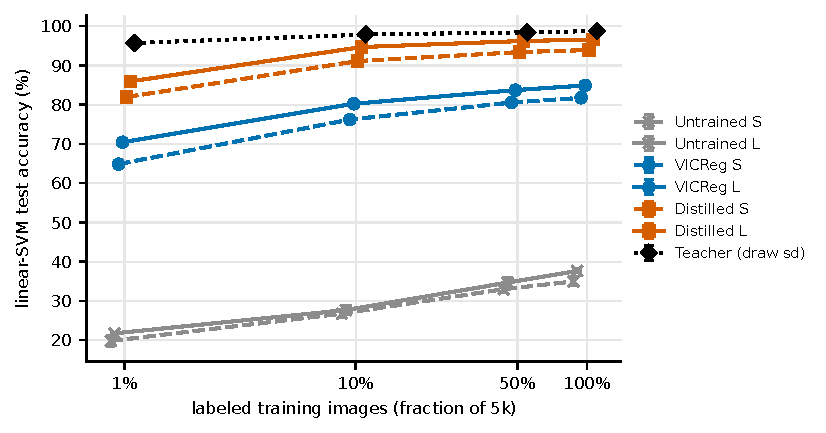
\includegraphics[width=0.48\linewidth]{figures/label_efficiency}\hfill
  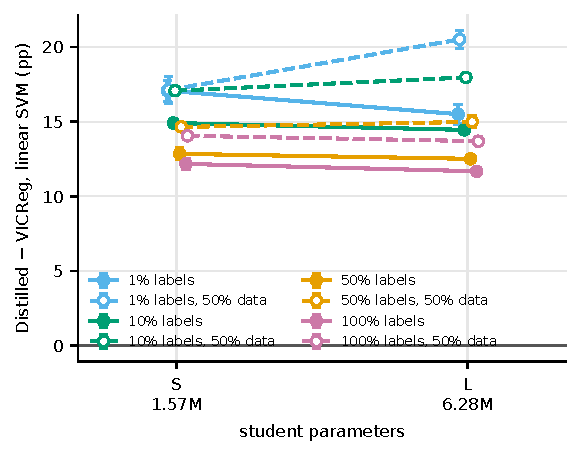
\includegraphics[width=0.48\linewidth]{figures/gap_vs_params}
% FIX: caption still uses letters (D, B, C, \CB). \CB is defined at the top of the file;
% redefining it as Distilled$-$VICReg fixes every caption that uses it at once.
  \caption{Left: label efficiency (linear SVM; error bars: seed sd; D: draw sd).
    Right: \CB{} gap (linear SVM) vs.\ student parameters, per label fraction and
    unlabeled-data setting (error bars: larger of B's and C's seed sd).}
  \label{fig:curves}
\end{figure}

\subsection{Q1: Does distillation beat direct training?}
\label{sec:q1}

% FIX: "This is expected since STL-10 is based on ImageNet" is stronger than the evidence:
% the overlap is a plausible explanation that EuroSAT supports, not a certainty (difficulty and
% resolution differ too). "in one experiment" -> at 1% labels (both sizes).
Yes. Almost every experiment run concluded so, how much is a better question. On STL-10 it is a very clear win for the distilled student. This is expected since STL-10 is based on ImageNet, which the teacher is based on. On EuroSAT, however, the gap is much narrower, and in one experiment the direct training ties or wins compared to distillation. This may indicate that an even more out-of-domain dataset could flip the results. The gap also narrows for the linear SVM classifier with more labeled data. On this budget, the direct trained student also seems to be undertrained, indicating that more training could also narrow the gap. 

\subsection{Q2: How much of the teacher survives compression?}
\label{sec:q2}

% Generated by `mo433 report`. Do not edit.
\begin{table}[t]
\centering
\small
\caption{Encoder cost at the native input size. GPU latency: RTX 3060 Laptop, batch 256, fp32 (ms per batch); CPU latency: batch 1, 16 threads (ms per image). MACs = FLOPs/2.}
\label{tab:costs}
\begin{tabular}{lrrrrrr}
\toprule
Encoder & Input px & Params (M) & GMACs & Dim & GPU ms & CPU ms \\
\midrule
ResNet96-S (students) & 96 & 1.57 & 0.18 & 192 & 23.2 & 2.4 \\
ResNet96-L (students) & 96 & 6.28 & 0.70 & 384 & 62.3 & 5.0 \\
ViT-S/16 (teacher) & 224 & 21.67 & 4.24 & 384 & 450.1 & 28.9 \\
\bottomrule
\end{tabular}
\par\smallskip{\footnotesize Probe capacity grows with the feature dimension, which differs between S and L/D.}
\end{table}


% FIX typos: seperability, handfew. "we may not want the teacher to survive" reads oddly; the
% point is that the student should not simply copy a teacher that is out of its domain.
Mostly. With all labels, the large distilled student reaches \AccCLFullLinHundred\% linear-SVM
accuracy against the teacher's \AccDLinHundred\%, and the small one \AccCSFullLinHundred\%. With fewer labels, however, less of the teacher survives. This indicates that the student can inherit some linearly decodable information, but can't grasp the desired class seperability needed with a handfew of examples. ARI and NMI numbers support this. In other domains, such as the EuroSAT images, we may not want the teacher to survive. The student ties with or beats the teacher on a few occasions, adapting to the domain while the teacher stayed frozen. The teacher only seems to be the ceiling inside its domain. 

\subsection{Q3: Was the detour worth it?}
\label{sec:q3}

% Generated by `mo433 report`. Do not edit.
\begin{table}[t]
\centering
\footnotesize
\caption{Training budget per run group (mean per run) and accuracy per GPU-hour (linear SVM, 100\% labels; Distilled is charged the teacher cache and the teacher's pretraining estimate).}
\label{tab:budget}
\begin{tabular}{lrrrrr}
\toprule
Group & Runs & GPU-h & Wall-h & Acc. & pp/GPU-h \\
\midrule
VICReg S, 100\% & 3 & 1.29 & 1.31 & 81.7 & 63.2 \\
Distilled S, 100\% & 3 & 0.49 & 0.51 & 93.9 & 0.0303 \\
VICReg S, 50\% & 3 & 0.64 & 0.66 & 78.7 & 123 \\
Distilled S, 50\% & 3 & 0.24 & 0.25 & 92.8 & 0.0299 \\
VICReg L, 100\% & 2 & 2.71 & 2.74 & 84.9 & 31.3 \\
Distilled L, 100\% & 2 & 1.22 & 1.24 & 96.6 & 0.0311 \\
VICReg L, 50\% & 2 & 1.35 & 1.38 & 81.6 & 60.6 \\
Distilled L, 50\% & 2 & 0.61 & 0.63 & 95.3 & 0.0307 \\
\midrule
\multicolumn{2}{l}{Total VICReg (GPU-h)} & 13.9 & & & \\
\multicolumn{2}{l}{Total distillation (GPU-h)} & 5.9 & & & \\
\multicolumn{2}{l}{Teacher cache, once (GPU-h)} & 0.83 & & & \\
\multicolumn{2}{l}{Distillation all-in incl.\ pretraining (GPU-h)} & 3{,}107 & & & \\
\multicolumn{2}{l}{Teacher pretraining (estimate)} & 3{,}100 & & & \\
\bottomrule
\end{tabular}
\par\smallskip{\footnotesize Teacher pretraining: 1.16k GPU-h for 300 epochs (DINO Table~8), extrapolated linearly to 800 epochs.}
\end{table}


% FIX: "orders of magnitude cheaper in both compute and data volume": the accounting is
% compute only, so drop "data volume". Typos: directly training, cheapset, defintely, "if have to".
% SUGGEST: a footnote with the two measurement notes (one VICReg epoch's impossible GPU time was
% capped at its wall time; the teacher cache was timed on a shared GPU, so it is overstated).
It depends on how you count it, especially whether we consider the pre-training budget into the equation. If we consider it, then the directly training is orders of magnitude cheaper in both compute and data volume. Otherwise, it reverses. Because the distilled student uses only 1 versus 2 seperate views like the VICReg, the distilled trains faster (and cheaper) than its competition, apart from being more accurate. Even when the longest-trained the VICReg with the 300-epoch runs of Section~\ref{sec:long300} didn't beat the cheapset distilled configuration. The detour is defintely worth it when a full free teacher checkpoint is available, but not if have to pretrain ourselves.

\subsection{Q4: Do the unsupervised diagnostics agree with the probes?}
\label{sec:q4}

% Generated by `mo433 report`. Do not edit.
\begin{table}[t]
\centering
\scriptsize
\caption{Unsupervised diagnostics, mean $\pm$ sd over seeds. Validation split: $k$-NN accuracy (\%), spread = per-dimension std $\times\sqrt{d}$, $k$-means NMI; test split: $k$-means NMI and ARI. Flagged: collapse check fired (count/encoders); D: teacher sanity check.}
\label{tab:diagnostics}
\begin{tabular}{lcccccc}
\toprule
Encoder & Val $k$-NN & Spread & Val NMI & Test NMI & Test ARI & Flagged \\
\midrule
A-S & 31.2 $\pm$ 2.6 & 0.09 $\pm$ 0.01 & 0.130 $\pm$ 0.014 & 0.090 $\pm$ 0.013 & 0.042 $\pm$ 0.003 & anchor \\
B-S, 100\% & 77.3 $\pm$ 0.6 & 0.72 $\pm$ 0.01 & 0.522 $\pm$ 0.010 & 0.535 $\pm$ 0.002 & 0.402 $\pm$ 0.006 & 0/3 \\
C-S, 100\% & 91.9 $\pm$ 0.6 & 0.49 $\pm$ 0.02 & 0.676 $\pm$ 0.016 & 0.688 $\pm$ 0.032 & 0.593 $\pm$ 0.074 & 0/3 \\
B-S, 50\% & 75.1 $\pm$ 0.8 & 0.71 $\pm$ 0.00 & 0.510 $\pm$ 0.016 & 0.503 $\pm$ 0.004 & 0.370 $\pm$ 0.008 & 0/3 \\
C-S, 50\% & 90.7 $\pm$ 0.1 & 0.50 $\pm$ 0.01 & 0.689 $\pm$ 0.018 & 0.672 $\pm$ 0.016 & 0.584 $\pm$ 0.021 & 0/3 \\
A-L & 34.7 $\pm$ 0.4 & 0.10 $\pm$ 0.01 & 0.132 $\pm$ 0.022 & 0.109 $\pm$ 0.004 & 0.055 $\pm$ 0.006 & anchor \\
B-L, 100\% & 82.1 $\pm$ 0.7 & 0.79 $\pm$ 0.00 & 0.560 $\pm$ 0.024 & 0.595 $\pm$ 0.011 & 0.457 $\pm$ 0.042 & 0/2 \\
C-L, 100\% & 95.3 $\pm$ 0.7 & 0.50 $\pm$ 0.04 & 0.785 $\pm$ 0.026 & 0.753 $\pm$ 0.043 & 0.677 $\pm$ 0.089 & 0/2 \\
B-L, 50\% & 78.0 $\pm$ 0.3 & 0.79 $\pm$ 0.00 & 0.514 $\pm$ 0.021 & 0.544 $\pm$ 0.004 & 0.402 $\pm$ 0.010 & 0/2 \\
C-L, 50\% & 94.5 $\pm$ 1.0 & 0.56 $\pm$ 0.00 & 0.735 $\pm$ 0.002 & 0.764 $\pm$ 0.040 & 0.693 $\pm$ 0.092 & 0/2 \\
D & 98.2 & 0.90 & 0.906 & 0.900 & 0.877 & pass \\
\bottomrule
\end{tabular}
\end{table}


\begin{figure}[t]
  \centering
  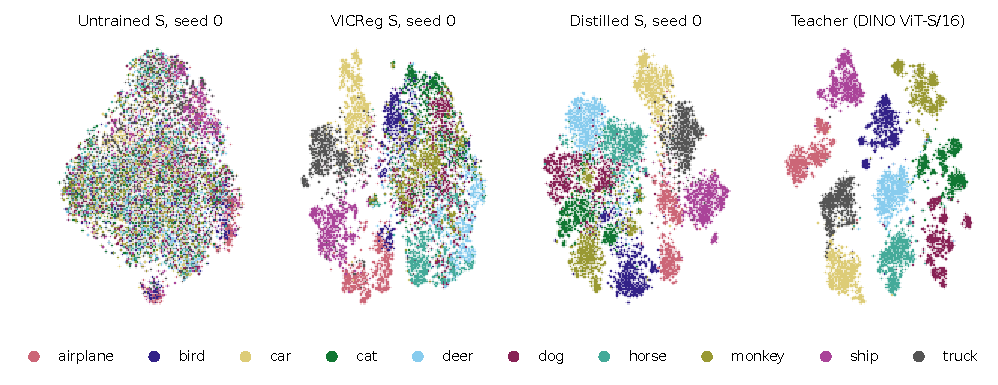
\includegraphics[width=\linewidth]{figures/tsne}
  \caption{t-SNE of test-split features for one encoder per row (seed 0, S, 100\% data;
    perplexity 30, \texttt{random\_state=0}), coloured by true class.}
  \label{fig:tsne}
\end{figure}

% FIX: "as we mentioned previously" points forward: EuroSAT comes later -> Section~\ref{sec:eurosat}.
% SUGGEST: one EuroSAT VICReg seed (S, 50% data) lost ~10 pp; its spread and NMI dropped, but it
% passed the collapse check, so the binary check only catches total collapse and the continuous
% diagnostics are the more informative signal. Good answer to "do the diagnostics agree".
Mostly yes. The ordering is preserved (Untrained < VICReg < Distilled < Teacher on all metrics in STL-10), but the spread is different. Since VICReg's variance term pushes each dimension's standard deviation up, compared to a single view matching with teacher in the distilled student, it is expected that the directly trained student presents higher spread. And as we mentioned previously, the out-of-domain order changes with the teacher dropping position, even behind VICReg.

The project brief also asks what changes when two encoders score the same on the SVM but differ in NMI. This is most visible across distinct seeds of the distilled student: the linear-SVM standard deviation of the large distilled student with 100\% data is \AccSdCLFullLinHundred~pp, while its test ARI varies by $\pm$\,0.09, its test NMI by $\pm$\,0.04. K-means uses fixed seeds, so k-means instability is unlikely to be the main source of the variation. Even then, a different geometry can land k-means in a different local optimum, so the variation probably comes from the encoders, but some of it may be amplified by k-means itself. 

\subsection{Q5: Does the gap change with student size?}
\label{sec:q5}

% FIX: "the error measured in pp" -> the gap in pp. "as size and data quantity increase": data was
% only reduced (ablation), never increased. Typos: sesm, detph.
Only slightly. As the table shows, the error measured in pp is pretty much flat across the two main sizes and the four of Section~\ref{sec:sizes}. VICReg doesn't come close to beating distillation. However, the distilled model has a significant improvement in performance in terms of error ratio against VICReg. The hypothesis that states that a directly trained student would eventually beat a distilled one as size and data quantity increase sesm to fail, at least at this scale. Then again, the VICReg student seems to be undertrained (Section~\ref{sec:q6}).

That being said, we only tested increasing the width of the network, not detph. Perhaps a deeper network (and more training) would give more concrete results.

\subsection{Ablation: unlabeled data and steps}
\label{sec:ablation}

% Generated by `mo433 report`. Do not edit.
\begin{table}[t]
\centering
\footnotesize
\caption{Ablation grid: C $-$ B gap (pp) per unlabeled-data setting $\times$ student size. The 50\% setting halves both the data and the optimizer steps.}
\label{tab:ablation}
\begin{tabular}{llcccc}
\toprule
Probe & Labels & S, 100\% data & S, 50\% data & L, 100\% data & L, 50\% data \\
\midrule
$k$-NN & 1\% & +14.3 (0.9)$^*$ & +14.8 (0.8)$^*$ & +13.4 (0.4)$^*$ & +17.2 (0.9)$^*$ \\
 & 10\% & +13.1 (0.2)$^*$ & +15.2 (0.5)$^*$ & +12.0 (0.1)$^*$ & +15.9 (0.2)$^*$ \\
 & 50\% & +13.8 (0.2)$^*$ & +15.6 (0.4)$^*$ & +12.6 (0.3)$^*$ & +16.0 (0.2)$^*$ \\
 & 100\% & +13.7 (0.3)$^*$ & +15.8 (0.2)$^*$ & +12.5 (0.1)$^*$ & +15.8 (0.4)$^*$ \\
\midrule
Linear SVM & 1\% & +17.1 (0.7)$^*$ & +17.1 (0.9)$^*$ & +15.5 (0.7)$^*$ & +20.5 (0.6)$^*$ \\
 & 10\% & +14.9 (0.2)$^*$ & +17.1 (0.3)$^*$ & +14.5 (0.2)$^*$ & +18.0 (0.1)$^*$ \\
 & 50\% & +12.8 (0.4)$^*$ & +14.7 (0.3)$^*$ & +12.5 (0.2)$^*$ & +15.0 (0.4)$^*$ \\
 & 100\% & +12.2 (0.4)$^*$ & +14.1 (0.2)$^*$ & +11.7 (0.2)$^*$ & +13.7 (0.3)$^*$ \\
\midrule
RBF SVM & 1\% & +14.1 (0.6)$^*$ & +14.8 (0.3)$^*$ & +13.6 (0.8)$^*$ & +16.8 (0.7)$^*$ \\
 & 10\% & +14.2 (0.1)$^*$ & +16.2 (0.5)$^*$ & +13.4 (0.2)$^*$ & +16.0 (0.3)$^*$ \\
 & 50\% & +12.3 (0.4)$^*$ & +14.3 (0.1)$^*$ & +11.4 (0.2)$^*$ & +13.7 (0.0)$^*$ \\
 & 100\% & +11.4 (0.4)$^*$ & +13.7 (0.2)$^*$ & +10.1 (0.4)$^*$ & +12.4 (0.4)$^*$ \\
\bottomrule
\end{tabular}
\par\smallskip{\footnotesize $\Delta$ = C $-$ B in pp, (reference sd = larger of B's and C's seed sd); $^*$ beyond spread, $|\Delta|$ $>$ reference sd.}
\end{table}


\begin{figure}[t]
  \centering
  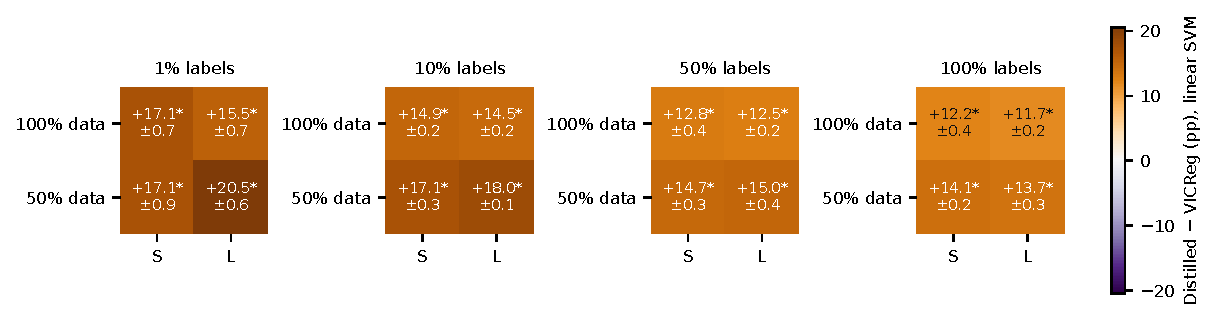
\includegraphics[width=0.6\linewidth]{figures/ablation_grid}
  \caption{Ablation grid: \CB{} gap per unlabeled-data setting $\times$ student size
    ($^*$ beyond spread).}
  \label{fig:ablation}
\end{figure}

\paragraph{What it tests.} The ablation trains VICReg and distillation on the 50k-image ablation subset
instead of all 100k images, for both sizes, same seeds, epochs and probes. Epochs
stay the same, so the 50\% runs also take half the optimizer steps, so the ablation varies a joint
data-and-compute budget, not data alone.

% FIX: "The larger networks are also more affected" is not supported: both sizes lose about the
% same; the extra widening for L shows only at 1% labels, on two seeds. "VICReg target" ->
% VICReg student. Typos: faver, "wins be".
Going into this, we expected that a smaller budget should faver distillation, since it has a teacher that supplies a good target for every image, while the other student has to learn from scratch. We confirm that in our findings. As we use less data, distillation wins be an ever-greater margin. This is mostly due to the VICReg target getting worse, while the distilled student better maintains its performance. The larger networks are also more affected by the decrease in data volume. 

\subsection{Eval-only multi-scale probe}
\label{sec:multiscale}

% FIX: "on all labels" reads as "at every label fraction", but the gain is only with 100% labels
% (none at 10%). Typos: dissapears, "features is".
Adding stage-3 features seems to help VICReg slightly on all labels, but that's as far as it goes. For the distilled student and VICReg with few labels, it doesn't help. Even on the smaller VICReg student, the gain dissapears as soon as the concatenated features is projected back to the original dimension. This means that it only reflects the extra probe capacity instead of actual extra information. For the larger student, it partly survives. In any case, intermediate features do not change the comparison between the students.

% Generated by `mo433 report`. Do not edit.
\begin{table}[t]
\centering
\footnotesize
\caption{Individual large-student (L) encoders: test accuracy (\%), mean over the 3 label draws.}
\label{tab:l-runs}
\begin{tabular}{lcccc}
\toprule
Encoder & 1\% & 10\% & 50\% & 100\% \\
\midrule
\multicolumn{5}{l}{\textit{$k$-NN}} \\
A-L-s0 & 20.4 & 25.7 & 31.3 & 33.5 \\
A-L-s1 & 20.7 & 27.4 & 31.9 & 33.2 \\
B-L-100-s0 & 63.9 & 78.1 & 81.3 & 82.2 \\
B-L-100-s1 & 64.1 & 78.1 & 81.3 & 82.1 \\
C-L-100-s0 & 77.7 & 90.0 & 93.7 & 94.6 \\
C-L-100-s1 & 77.1 & 90.2 & 94.1 & 94.7 \\
B-L-050-s0 & 61.1 & 74.3 & 77.7 & 78.9 \\
B-L-050-s1 & 59.9 & 73.9 & 77.4 & 78.3 \\
C-L-050-s0 & 77.4 & 89.9 & 93.5 & 94.4 \\
C-L-050-s1 & 77.9 & 90.1 & 93.5 & 94.3 \\
\midrule
\multicolumn{5}{l}{\textit{Linear SVM}} \\
A-L-s0 & 21.7 & 28.5 & 35.6 & 38.0 \\
A-L-s1 & 21.8 & 26.9 & 33.7 & 37.3 \\
B-L-100-s0 & 70.4 & 80.2 & 83.8 & 85.0 \\
B-L-100-s1 & 70.4 & 80.2 & 83.7 & 84.8 \\
C-L-100-s0 & 85.5 & 94.5 & 96.1 & 96.5 \\
C-L-100-s1 & 86.4 & 94.8 & 96.3 & 96.6 \\
B-L-050-s0 & 65.8 & 75.4 & 80.3 & 81.7 \\
B-L-050-s1 & 65.0 & 75.3 & 79.7 & 81.5 \\
C-L-050-s0 & 85.5 & 93.3 & 95.0 & 95.1 \\
C-L-050-s1 & 86.3 & 93.3 & 95.0 & 95.5 \\
\midrule
\multicolumn{5}{l}{\textit{RBF SVM}} \\
A-L-s0 & 23.2 & 33.2 & 39.9 & 42.2 \\
A-L-s1 & 23.5 & 33.5 & 39.9 & 42.0 \\
B-L-100-s0 & 67.7 & 80.2 & 84.7 & 86.7 \\
B-L-100-s1 & 66.5 & 79.9 & 84.5 & 86.1 \\
C-L-100-s0 & 80.5 & 93.3 & 95.9 & 96.5 \\
C-L-100-s1 & 81.0 & 93.6 & 96.1 & 96.5 \\
B-L-050-s0 & 64.8 & 76.6 & 81.3 & 83.5 \\
B-L-050-s1 & 63.8 & 76.4 & 81.2 & 82.9 \\
C-L-050-s0 & 81.3 & 92.7 & 95.0 & 95.6 \\
C-L-050-s1 & 80.9 & 92.3 & 94.9 & 95.5 \\
\bottomrule
\end{tabular}
\end{table}

% Generated by `mo433 report`. Do not edit.
\begin{table}[t]
\centering
\scriptsize
\caption{Eval-only multi-scale probe (linear SVM, test accuracy \%): main feature, concatenated GAP(stage 3)+GAP(stage 4), and its fixed random projection to the main dimension.}
\label{tab:multiscale}
\begin{tabular}{lcccccc}
\toprule
Encoder & main, 10\% & s3+s4, 10\% & s3+s4 proj., 10\% & main, 100\% & s3+s4, 100\% & s3+s4 proj., 100\% \\
\midrule
A-S & 26.8 $\pm$ 1.0 & 28.3 $\pm$ 1.0 & 28.5 $\pm$ 1.4 & 35.0 $\pm$ 1.1 & 38.2 $\pm$ 1.3 & 37.3 $\pm$ 1.2 \\
B-S, 100\% & 76.2 $\pm$ 0.2 & 76.0 $\pm$ 0.3 & 75.1 $\pm$ 0.2 & 81.7 $\pm$ 0.4 & 82.6 $\pm$ 0.4 & 81.6 $\pm$ 0.5 \\
C-S, 100\% & 91.1 $\pm$ 0.2 & 90.7 $\pm$ 0.2 & 89.1 $\pm$ 0.1 & 93.9 $\pm$ 0.2 & 93.8 $\pm$ 0.2 & 92.8 $\pm$ 0.3 \\
B-S, 50\% & 72.6 $\pm$ 0.3 & 72.8 $\pm$ 0.3 & 71.6 $\pm$ 0.1 & 78.7 $\pm$ 0.2 & 79.9 $\pm$ 0.4 & 78.8 $\pm$ 0.6 \\
C-S, 50\% & 89.7 $\pm$ 0.2 & 89.3 $\pm$ 0.1 & 87.7 $\pm$ 0.2 & 92.8 $\pm$ 0.1 & 92.7 $\pm$ 0.2 & 91.8 $\pm$ 0.2 \\
A-L & 27.7 $\pm$ 1.1 & 28.8 $\pm$ 0.9 & 29.7 $\pm$ 0.5 & 37.6 $\pm$ 0.5 & 40.6 $\pm$ 0.7 & 40.3 $\pm$ 0.3 \\
B-L, 100\% & 80.2 $\pm$ 0.0 & 80.2 $\pm$ 0.1 & 79.4 $\pm$ 0.4 & 84.9 $\pm$ 0.2 & 86.0 $\pm$ 0.0 & 85.6 $\pm$ 0.2 \\
C-L, 100\% & 94.7 $\pm$ 0.2 & 94.4 $\pm$ 0.3 & 94.0 $\pm$ 0.2 & 96.6 $\pm$ 0.1 & 96.5 $\pm$ 0.0 & 96.3 $\pm$ 0.1 \\
B-L, 50\% & 75.3 $\pm$ 0.1 & 75.6 $\pm$ 0.3 & 75.0 $\pm$ 0.3 & 81.6 $\pm$ 0.1 & 82.7 $\pm$ 0.2 & 82.5 $\pm$ 0.3 \\
C-L, 50\% & 93.3 $\pm$ 0.0 & 93.0 $\pm$ 0.1 & 92.2 $\pm$ 0.0 & 95.3 $\pm$ 0.3 & 95.2 $\pm$ 0.3 & 94.9 $\pm$ 0.1 \\
\bottomrule
\end{tabular}
\end{table}


% =====================================================================================
\section{Extra experiments (after the freeze)}
\label{sec:extras}

% SUGGEST: say they ran after the freeze, untuned, and are reported separately from the main study.
Beyond the initial 20 runs, we ran four extra experiments using the frozen configurations. This involved a second, out-of-domain dataset (EuroSAT), more student sizes, longer training, and an additional LeJEPA objective student to compare against VICReg and distillation.

\subsection{Second dataset: EuroSAT}
\label{sec:eurosat}

% Generated by `mo433 report-extras`. Do not edit.
\begin{table}[t]
\centering
\small
\caption{Linear-SVM test accuracy (\%) on STL-10 and EuroSAT with three direct or distilled objectives for the S student (100\% unlabeled data, frozen settings). VICReg and Distilled: 3 seeds; LeJEPA (extra experiment): 2 seeds; Teacher: sd over label draws.}
\label{tab:extras-datasets}
\begin{tabular}{lcccccc}
\toprule
\multicolumn{1}{l}{} & \multicolumn{3}{c}{STL-10} & \multicolumn{3}{c}{EuroSAT} \\
\cmidrule(lr){2-4}\cmidrule(lr){5-7}
S student & 1\% & 10\% & 100\% & 1\% & 10\% & 100\% \\
\midrule
Untrained & 19.8 $\pm$ 1.3 & 26.8 $\pm$ 1.0 & 35.0 $\pm$ 1.1 & 34.9 $\pm$ 1.9 & 45.6 $\pm$ 2.2 & 56.2 $\pm$ 1.2 \\
VICReg & 64.9 $\pm$ 0.7 & 76.2 $\pm$ 0.2 & 81.7 $\pm$ 0.4 & 85.7 $\pm$ 0.3 & 91.7 $\pm$ 0.2 & 93.8 $\pm$ 0.0 \\
LeJEPA & 64.7 $\pm$ 0.2 & 74.6 $\pm$ 0.6 & 80.4 $\pm$ 0.2 & 82.5 $\pm$ 0.3 & 89.2 $\pm$ 0.3 & 91.9 $\pm$ 0.4 \\
Distilled & 81.9 $\pm$ 0.1 & 91.1 $\pm$ 0.2 & 93.9 $\pm$ 0.2 & 85.3 $\pm$ 0.7 & 94.2 $\pm$ 0.3 & 96.4 $\pm$ 0.1 \\
Teacher & 95.7 $\pm$ 0.4 & 97.9 $\pm$ 0.2 & 98.8 $\pm$ 0.0 & 83.4 $\pm$ 1.0 & 92.8 $\pm$ 0.4 & 96.3 $\pm$ 0.0 \\
\midrule
$\Delta$ Distilled $-$ VICReg & +17.1 (0.7)$^*$ & +14.9 (0.2)$^*$ & +12.2 (0.4)$^*$ & \ensuremath{-}0.4 (0.7) & +2.4 (0.3)$^*$ & +2.6 (0.1)$^*$ \\
$\Delta$ LeJEPA $-$ VICReg & \ensuremath{-}0.2 (0.7) & \ensuremath{-}1.6 (0.6)$^*$ & \ensuremath{-}1.4 (0.4)$^*$ & \ensuremath{-}3.2 (0.3)$^*$ & \ensuremath{-}2.5 (0.3)$^*$ & \ensuremath{-}1.9 (0.4)$^*$ \\
$\Delta$ Distilled $-$ LeJEPA & +17.3 (0.2)$^*$ & +16.5 (0.6)$^*$ & +13.5 (0.2)$^*$ & +2.8 (0.7)$^*$ & +4.9 (0.3)$^*$ & +4.5 (0.4)$^*$ \\
\bottomrule
\end{tabular}
\par\smallskip{\footnotesize $\Delta$: gaps in percentage points with max(sd) in parentheses; $^*$ = larger than the seed-to-seed spread.}
\end{table}


\begin{figure}[t]
  \centering
  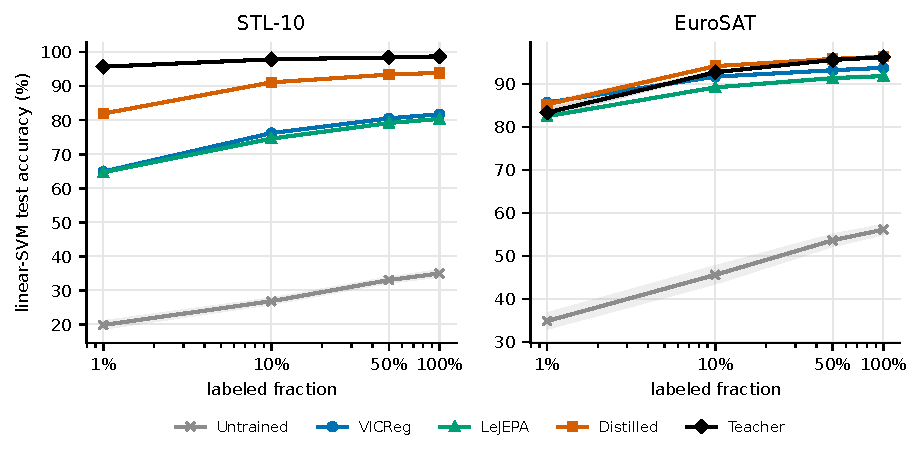
\includegraphics[width=\linewidth]{figures/extras_label_efficiency}
% FIX: caption still says "J (LeJEPA)".
  \caption{Label efficiency of the S student on STL-10 (left) and EuroSAT (right), linear
  SVM, mean $\pm$ sd over seeds. J (LeJEPA) is an extra experiment.}
  \label{fig:extras-label-efficiency}
\end{figure}

% FIX: "a stratified 5% subset" is wrong: it is a 5k (5,000-image) subset of the 21.6k training
% images, matching STL-10's 5k labeled set. "the teacher loses some advantage" is a result, not
% setup. Add: the full study was rerun with the frozen settings and the teacher passed its sanity
% check. Typos: iamges, startified, "teacher teacher", proves, "Since, this".
\paragraph{Setup.} EuroSAT RGB~\citep{helber2019eurosat} is comprised of 27k satellite iamges of 10 classes, each a different use of land. Since, this is very distinct from the ImageNet images, the teacher teacher loses some advantage. Since the dataset has no official train/test split, we used a startified 80\% for training, and the remaining 20\% for test. The unlabeled set was comprised of the entire training set(labels removed), with a stratified 5\% subset for the proves. To match the input, the 64$\times$64 images had to be upscaled to 96$\times$96 pixels. 

% SUGGEST: add (i) VICReg ties/wins at 1% labels; (ii) part of the STL-10 gap likely comes from
% the teacher's ImageNet exposure (links to Confounds); (iii) caveats: the teacher sees heavily
% upsampled 64 px images; one VICReg run (S, 50% data) partly failed, inflating that cell.
% Typos: "as that", comapred.
\paragraph{Results.} Out of the teacher's domain, distillation's advantage against VICReg shrinks significantly, and so does the teacher's. In this setup, both the distilled and VICReg student were able to match or even outperform the teacher with few labels. With all labels, distilled student is still able to match teacher performance. One caveat of these results as that EuroSAT is an easier task, as even the untrained student was able to get better performance comapred with the STL-10 dataset.

\subsection{A second direct method: LeJEPA}
\label{sec:lejepa}

% FIX: "our hypothesis that distilled always beats trained from scratch": "always" contradicts
% EuroSAT at 1% labels, and the brief's hypothesis is a crossover, not "always". Say LeJEPA tests
% whether the gap is specific to VICReg. SUGGEST: setup in one line (reference defaults, 2 views
% instead of the paper's multi-crop, S student, 2 seeds).
To explore more training methods, we copied the VICReg student configuration and swapped the objective with LeJEPA's~\citep{balestriero2025lejepa}, which regularizes the embedding towards an isotropic Gaussian, to directly train a student. This not only gives on opportunity to compare VICReg against LeJEPA, but also increases the robustness of our hypothesis that distilled always beats trained from scratch.

% FIX: "on either dataset on either datset" (duplicate); typos confidance, comparitvely.
% SUGGEST: the EuroSAT point worth making: there, swapping VICReg for LeJEPA roughly doubles the
% gap, so out of domain the choice of direct method matters about as much as distillation.
LeJEPA did not beat VICReg on either dataset on either datset, and was slightly worse overall. The gap between distilled and directly trained barely change on STL-10, which gives us more confidance that distillation still beats a comparable generic directly trained student. In EuroSAT, LeJEPA performed comparitvely worse than in STL-10. This should be taken with a grain of salt though, as LeJEPA was trained on an optimizer tuned for VICReg, so it is not its best performance.

\subsection{Longer training ($E=300$)}
\label{sec:long300}

% Generated by `mo433 report-extras`. Do not edit.
\begin{table}[t]
\centering
\small
\caption{Longer training (extra experiment): linear-SVM test accuracy (\%) of the S student at $E=100$ (main study, seeds 0--1 only) and $E=300$ (seeds 0--1), 100\% unlabeled data, STL-10.}
\label{tab:extras-long300}
\begin{tabular}{lcccc}
\toprule
Encoder & 1\% & 10\% & 50\% & 100\% \\
\midrule
VICReg, $E=100$ & 64.8 $\pm$ 1.0 & 76.2 $\pm$ 0.3 & 80.6 $\pm$ 0.5 & 81.8 $\pm$ 0.5 \\
VICReg, $E=300$ & 68.8 $\pm$ 0.1 & 78.8 $\pm$ 0.1 & 83.2 $\pm$ 0.1 & 84.4 $\pm$ 0.2 \\
Distilled, $E=100$ & 81.9 $\pm$ 0.2 & 91.1 $\pm$ 0.3 & 93.3 $\pm$ 0.1 & 93.9 $\pm$ 0.2 \\
Distilled, $E=300$ & 83.0 $\pm$ 0.6 & 92.4 $\pm$ 0.2 & 94.0 $\pm$ 0.0 & 94.3 $\pm$ 0.1 \\
\midrule
$\Delta$ Distilled $-$ VICReg, $E=100$ & +17.1 (1.0)$^*$ & +14.9 (0.3)$^*$ & +12.7 (0.5)$^*$ & +12.1 (0.5)$^*$ \\
$\Delta$ Distilled $-$ VICReg, $E=300$ & +14.1 (0.6)$^*$ & +13.5 (0.2)$^*$ & +10.7 (0.1)$^*$ & +9.9 (0.2)$^*$ \\
\bottomrule
\end{tabular}
\par\smallskip{\footnotesize $\Delta$: gaps in percentage points with max(sd) in parentheses; $^*$ = larger than the seed-to-seed spread.}
\end{table}


\begin{figure}[t]
  \centering
  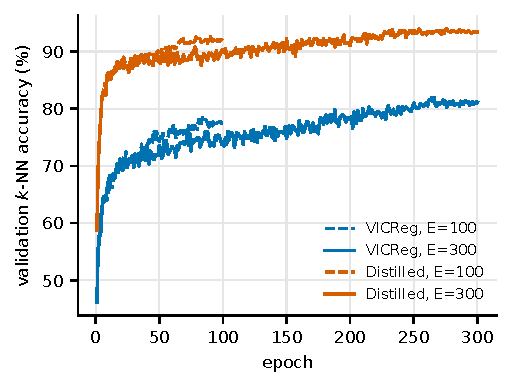
\includegraphics[width=0.55\linewidth]{figures/extras_long300_curves}
  \caption{Validation $k$-NN during training, S student, STL-10, mean of seeds 0--1:
  frozen budget ($E=100$, dashed) vs.\ $E=300$ (solid).}
  \label{fig:extras-long300-curves}
\end{figure}

% FIX typos: tripple, epocks, compareable, stretchs, "important to note, that".
% SUGGEST: mention 2 seeds, S only.
Extended training on the small student showed us that we could have squeezed more performance out of VICReg. With tripple the epocks, VICReg improved double the amount that the distilled student did. At this point, the distilled student's training curve has pretty much plateaued, while VICReg is still improving. This indicates that the distilled student learns faster, but is limited by its capacity (which larger students relieve - Section~\ref{sec:sizes}), and VICReg is limited by the training budget. For VICReg to surpass distillation, we would need much more training than a laptop GPU could offer. It is important to note, that only the endpoints are compareable with the original training because the cosine schedule stretchs as the run length grows. 

\subsection{More student sizes}
\label{sec:sizes}

% Generated by `mo433 report-extras`. Do not edit.
\begin{table}[t]
\centering
\small
\caption{Four student sizes (XS and M are extra experiments): linear-SVM test accuracy (\%) on STL-10, 100\% unlabeled data, $E=100$. XS, M and L: 2 seeds; S: 3 seeds. Widths 12/24/34/48, same scaling rule.}
\label{tab:extras-sizes}
\begin{tabular}{lrccccccccc}
\toprule
\multicolumn{1}{l}{} & \multicolumn{1}{l}{} & \multicolumn{3}{c}{1\% labels} & \multicolumn{3}{c}{10\% labels} & \multicolumn{3}{c}{100\% labels} \\
\cmidrule(lr){3-5}\cmidrule(lr){6-8}\cmidrule(lr){9-11}
Size & Params (M) & B & C & $\Delta$ & B & C & $\Delta$ & B & C & $\Delta$ \\
\midrule
XS & 0.39 & 59.2 & 72.3 & +13.1 (1.0)$^*$ & 70.2 & 85.1 & +14.9 (0.5)$^*$ & 75.5 & 89.1 & +13.6 (0.3)$^*$ \\
S & 1.57 & 64.9 & 81.9 & +17.1 (0.7)$^*$ & 76.2 & 91.1 & +14.9 (0.2)$^*$ & 81.7 & 93.9 & +12.2 (0.4)$^*$ \\
M & 3.15 & 68.4 & 83.2 & +14.8 (0.2)$^*$ & 78.4 & 93.2 & +14.7 (0.2)$^*$ & 83.8 & 95.5 & +11.7 (0.3)$^*$ \\
L & 6.28 & 70.4 & 85.9 & +15.5 (0.7)$^*$ & 80.2 & 94.7 & +14.5 (0.2)$^*$ & 84.9 & 96.6 & +11.7 (0.2)$^*$ \\
\bottomrule
\end{tabular}
\par\smallskip{\footnotesize Gaps in percentage points with max(sd) in parentheses; $^*$ = larger than the seed-to-seed spread.}
\end{table}


\begin{figure}[t]
  \centering
  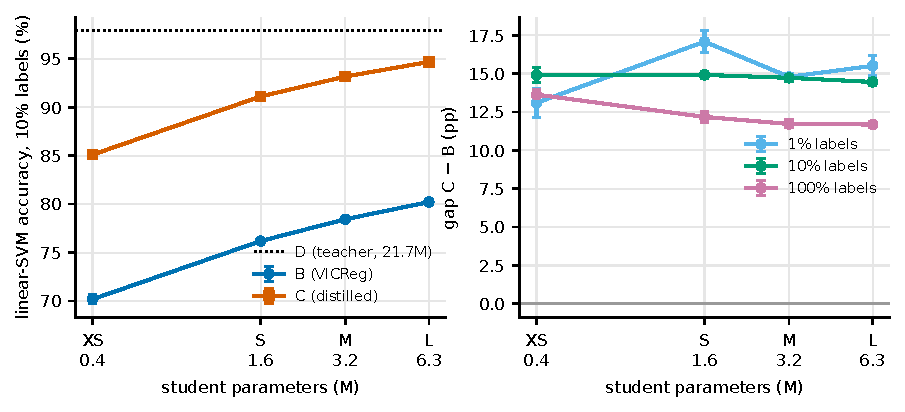
\includegraphics[width=\linewidth]{figures/extras_sizes}
  \caption{Four student sizes on STL-10 (XS and M are extra experiments). Left: linear-SVM
  accuracy at 10\% labels against parameters. Right: gap distilled$-$VICReg against parameters for three
  label fractions; error bars are the larger of the two seed sds.}
  \label{fig:extras-sizes}
\end{figure}

% FIX: "improved with size at the same rate as the other sizes" -> both methods improve with size
% at about the same rate; "no significant distance in the gap" -> the gap stays almost constant;
% "ahead the most expensive" -> ahead of the largest.
Two more sizes (XS and M) were built with the same width rule and extend the range to sixteen-fold in parameter count. The methods improved with size at the same rate as the other sizes, so there is no significant distance in the gap between distilled and VICReg students on few labels, with a slight reduction when all labels were used. Even the smallest distillation is healthily ahead the most expensive VICReg student with few labels, with absolutely no sign of a crossover at this scale.

% =====================================================================================
\section{Difficulties and solutions}
\label{sec:difficulties}

The main practical constraint was the hardware. All training ran on a single 6 GB laptop GPU, which could not hold two training jobs at once, and the laptop's system memory was also limited. Its out-of-memory killer terminated our training a few times. We therefore ran every job sequentially as a memory-capped background service, with checkpoints so any run could resume after a failure. Throughput was also a difficulty. Generating augmented views on the fly made data loading unviable, so we had to precompute a pool of 20 augmented views per image and read them in shuffled chunks. A control run showed that there was barely a performance loss in validation k-NN, so we kept the pooled views. For the distilled student, running the ViT-S/16 teacher at every step would have exploded the cost. Instead, we cached its features once per pool view and checked the cache against live teacher outputs. Fairness under a limited tuning budget was another difficulty in methodology. We ran a single Optuna study, with median pruning of bad trials, on VICReg only and froze its winner for every other student, so the comparison does not favour distillation, which was the expected winner from the hypothesis.

The second dataset brought its own problems. EuroSAT has no official test split and its images are 64×64. We built a stratified 80/20 split and upsampled the images to 96×96, so the students and augmentations stayed fixed. Fitting the RBF SVM on all 21.6k training images took more than 15 minutes per encoder. We therefore probed on a stratified 5,000-image labeled subset, which keeps the label fractions comparable between the two datasets.

\section{Discussion}
\label{sec:discussion}

\subsection{Q6: Undertrained at this scale}
\label{sec:q6}

% FIX (not yet rewritten by you): this paragraph is the old draft (row letters B/C) and predates
% E=300. Rewrite it around Section~\ref{sec:long300}: VICReg gains about twice as much from 3x
% epochs, the gap narrows slowly and stays large.
All runs are short by self-supervised standards (100 epochs on 100k or 50k images, batch
256), and the results should be read as properties of this budget, not of the methods at
convergence. Two committed measurements suggest that B is further from convergence than C.
From the 20-epoch tuning runs to the 100-epoch reported runs (same configuration, S, 100\%
data), B's validation $k$-NN rises from 72.4\% (\texttt{tuning/grid\_B.json}, width 2048,
seeds 0--1) to \ValKnnBSFull\% (seeds 0--2), while C's rises only from 89.7\%
(\texttt{tuning/grid\_C.json}) to \ValKnnCSFull\%; and halving the budget costs B about three
times as much accuracy as C (Section~\ref{sec:ablation}). Both point the same way: with
longer training or more data, B would likely gain more than C, and the gap would shrink.
Whether it would close cannot be inferred from these runs.
\todo{update: the $E=300$ extra (Section~\ref{sec:long300}) now measures this.}
The size of the gap, especially
at 100\% labels, should be interpreted with this, and with the teacher's exposure to
ImageNet (below), in mind.

% FIX typo: "important to not that".
Since we previously observed that there was some undertraining, it is important to not that these results are limited to this compute budget, not the overall methods at their best. 

\subsection{Confounds}
\label{sec:confounds}

\begin{itemize}
% FIX (not yet rewritten by you): bullets still use row letters; the two red TODOs below are
% open. "Fixed views ... measured in Section~\ref{sec:limitations}" now points to the wrong
% place: the fixed-view control is in Section~\ref{sec:tuning}.
  \item \textbf{Supervision source and objective.} C and B differ both in where the signal
    comes from (a frozen teacher vs.\ the student's own views) and in the objective (cosine
    distillation of a DINO-trained teacher vs.\ VICReg), so the gap cannot be attributed to
    distillation alone. A DINO-trained convnet in B would remove the second difference; we
    did not run it because DINO is costlier and more collapse-prone at small budgets.
    \todo{add: LeJEPA (row J, Section~\ref{sec:lejepa}) as a second direct objective.}
  \item \textbf{ImageNet overlap.} STL-10 images come from ImageNet, which the teacher saw
    (without labels) during pretraining. This favours C and D and may explain part of the
    teacher's \AccDLinHundred\% and of C's margin; we discuss it but did not run a second,
    non-ImageNet dataset. \todo{WRONG NOW: EuroSAT was run (Section~\ref{sec:eurosat}); rewrite.}
  \item \textbf{Optimizer tuned on B.} The optimizer was tuned on B and copied to C, which
    biases the comparison toward B; a C win is therefore conservative in this respect.
  \item \textbf{Fixed views.} B and C train on the same 20 views per image; the cost of this
    for B is measured in Section~\ref{sec:limitations}.
  \item \textbf{Data and steps.} The ablation halves data and optimizer steps together
    (Section~\ref{sec:ablation}).
\end{itemize}

\subsection{Limitations}
\label{sec:limitations}

% FIX: "no significant change in student size" is wrong: four sizes over a 16x range.
% SUGGEST: restore the limitations that were dropped: the tuning proxy (20-epoch trials, best LR at
% the edge of the search space), fixed views (one-pair control), L and all extras on 2 seeds,
% extras untuned, the collapse check catching only total collapse.
Since we covered more than one student objective, and dataset, the main limitations are that there were no extra teachers analyzed, no significant change in student size and limited training runs. This is mostly due to time and compute constraints. Without them, we could do more optuna studies, compare more teachers, use on-the-fly augmentation, compare more seeds and run training until convergence.  

\section{Use of generative AI tools}
\label{sec:genai}

% =====================================================================================

% FIX: the course requires naming which code parts or steps used AI. One line is thin: list the
% parts (pipeline, training loops, probes, report generator, extras, tests), what you decided
% yourself, and how correctness was checked (unit tests, sanity checks). Also state that AI drafts
% were used as starting points for some report sections that you then rewrote, and which ones.
AI tools were useful in coding the training scripts at the student's (the author, not the model) discretion, as well as organizing the repository and revising the final report. 
\clearpage
\section{Conclusion}
\label{sec:conclusion}

% FIX: this is the old conclusion paragraph; your new one is below. Delete this one.
At the scale a single laptop GPU allows, distilling a frozen DINO ViT-S/16 into a small
ResNet beats training it with VICReg by 10--20~pp at every label fraction, for both student
sizes and both data amounts, and the advantage grows when unlabeled data and steps are
halved. The gap shrinks only marginally from 1.57M to 6.28M parameters, so the crossover
predicted by the brief lies, if anywhere, beyond the tested sizes, data and epochs. Whether
the detour is ``worth it'' depends entirely on accounting: with the teacher's pretraining
charged, direct training is about three orders of magnitude more efficient per GPU-hour;
with a public checkpoint treated as free, distillation gives more accuracy per GPU-hour in
three of four settings. These conclusions hold for VICReg as the direct method, on an
ImageNet-derived dataset, and at a budget at which B is likely undertrained.

% FIX typos: significantlly, definetely; "at few levels" -> with few labels; "beats training
% by far" -> beats direct training.
At our laptop GPU scale, distilling a frozen DINO ViT-S/16 into a small ResNet almost always beats training by far, especially if the target dataset is in the same domain as the teacher's pretraining. This holds true across different student sizes, data volume, training length and even the training objective, as LeJEPA does no better than VICReg. On a different domain, however, the advantage shrinks significantlly, especially at few levels. If a pretrained large model checkpoint is available to you, it is definetely worth it to distill rather than train from scratch. If you would have to do the pretraining yourself though, the detour is probably not worth it.

\paragraph{Reproducibility.} The repository regenerates every table and figure from the
frozen configurations with the command \texttt{uv run mo433 all}; the 20 final checkpoints are
published as a release. \todo{link the repository and the checkpoint release}

\subsection{Suggestions for improvement}
\label{sec:suggestions}

% FIX typos: convenet, ouf-of-domain; "could also test as stronger baseline narrowing the gap
% between distillation" is garbled. SUGGEST adding: patch-token distillation, longer training (also
% on EuroSAT), more seeds.
Introducing a DINO-trained convenet as another direct method would further clarify the difference in objective against the teacher. Optimizing as much as we can each direct method (instead of relying on VICReg's configuration for all students), and running LeJEPA with multi-crop could also test as stronger baseline narrowing the gap between distillation, especially in the ouf-of-domain EuroSAT dataset. A second teacher such as MAE and a teacher pretrained on EuroSAT's domain would help understand the impact of training method versus domain. 

% =====================================================================================
{\small
\setlength{\bibsep}{2pt}
\bibliographystyle{plainnat}
\bibliography{refs}
}

\end{document}
